\documentclass[main.tex]{subfiles}
\begin{document}

\href{https://www2.seas.gwu.edu/~simhaweb/quantum/modules/module8/module8.html}{Module 8: Quantum circuits - reversible construction}

\subsection{What is reversible construction?}

    Let's first describe what is meant by this term at a high-level, and then ask why it's useful. Steps in reversible construction: The starting point is: a computational problem we'd like to solve. Step 1: Solve the problem classically using a classical (Boolean) circuit shown in Figure \ref{fig:01reversible}.
    
    \begin{figure}
        \centering
        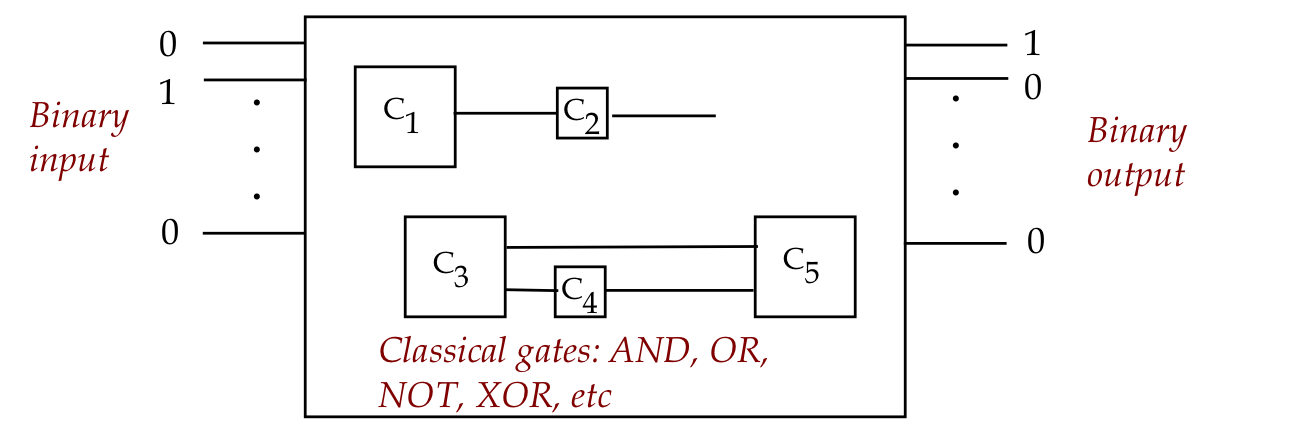
\includegraphics[width=5in]{notes/figs/n10/01reversible1.png}
        \caption{Classical (Boolean) Circuit}
        \label{fig:01reversible}
    \end{figure}
    
    Step 2: Replace the classical gates with classical reversible versions shown in Figure \ref{fig:02reversible2}.
    
    \begin{figure}
        \centering
        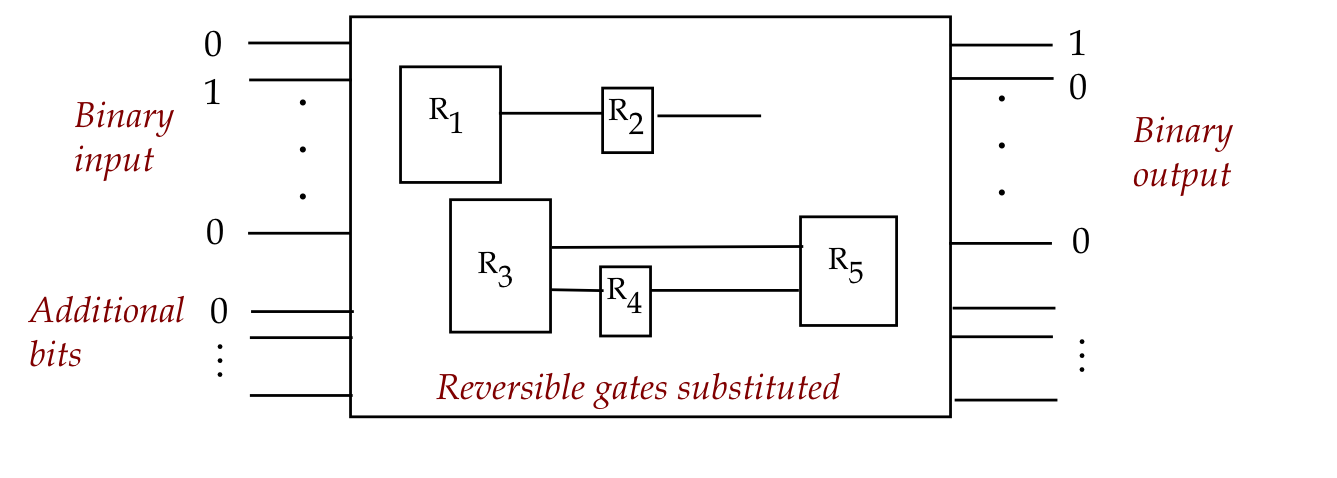
\includegraphics[width=5in]{notes/figs/n10/02reversible2.png}
        \caption{Classical reversible versions}
        \label{fig:02reversible2}
    \end{figure}
    
    Here, each classical gate $C_{i}$ is replaced by a reversible equivalent $R_{i}$. The reversible ones are typically larger (more inputs and outputs). Step 3: Substitute quantum (reversible) equivalents of the reversible classical gates, and use qubits shown in Figure \ref{fig:03reversible3}.
    
    \begin{figure}
        \centering
        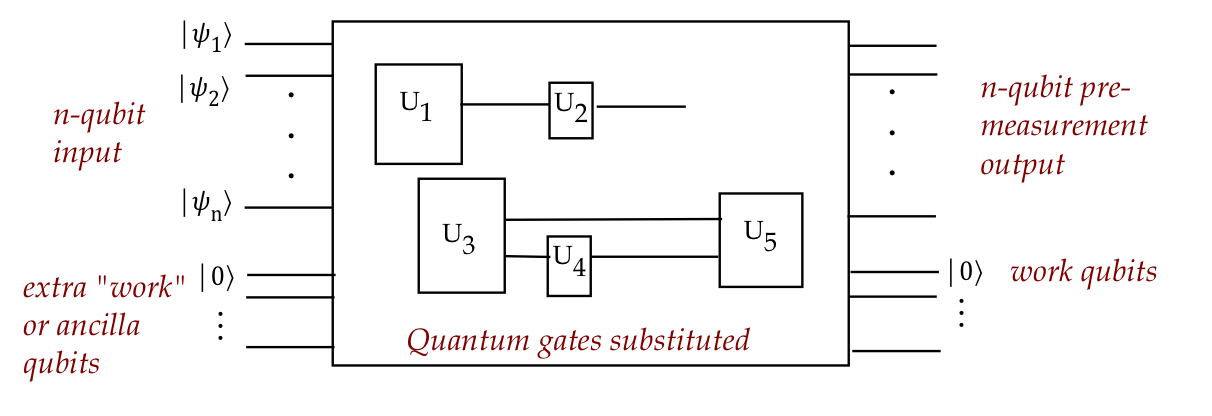
\includegraphics[width=5in]{notes/figs/n10/03reversible3.png}
        \caption{Quantum (reversible) equivalents}
        \label{fig:03reversible3}
    \end{figure}
    
    Quantum gates are already reversible (unitaries are invertible). Step 4: Optionally, optimize the quantum circuit. Terminology: the extra "work space qubits" are often called ancillae qubits (Singular: ancilla). Let's ask: why construct a quantum circuit of the same size if a classical circuit solves a problem? The answer: we can feed as input a superposition of all standard-basis vectors:
    
    $$
    \left|\psi_{\text {input }}\right\rangle=\frac{1}{\sqrt{N}} \sum_{i}|i\rangle=\frac{1}{\sqrt{N}}(|00 \ldots 0\rangle+\ldots+|11 \ldots 1\rangle)
    $$
    
    The hope is that the quantum circuit can act on all in parallel. However: we need to measure at the end. Measurement will result in only one output. And this too is random. Thus, one needs more than the reversible construction: Additional circuitry is needed to arrange for some desired outputs to occur with higher probability. Interference! Why consider this approach? This is one of three high-level approaches to quantum circuit: 1. Crafting circuits by hand. 2. Algorithmically converting a giant unitary into circuits with as few gates as possible. 3. Reversible construction. So far, only the first approach has been successful. There is on-going work in the second. The third, the reversible approach, at least provides a starting point that one can further optimize. Also, even hand-crafted quantum circuits make use of building blocks: For example: an adder. These can be implemented via classical circuits and then optimized. The reversible approach also proves that a quantum circuit can, with low overhead, implement a classical circuit.
    
\subsection{Binary-variable notation}

    It will be convenient to introduce some notational conventions for binary variables, to be used in three situations. First: we use them to describe Boolean gates: Example: the classical NOT gate shown in Figure \ref{fig:04classical-not}.
    
    \begin{figure}
        \centering
        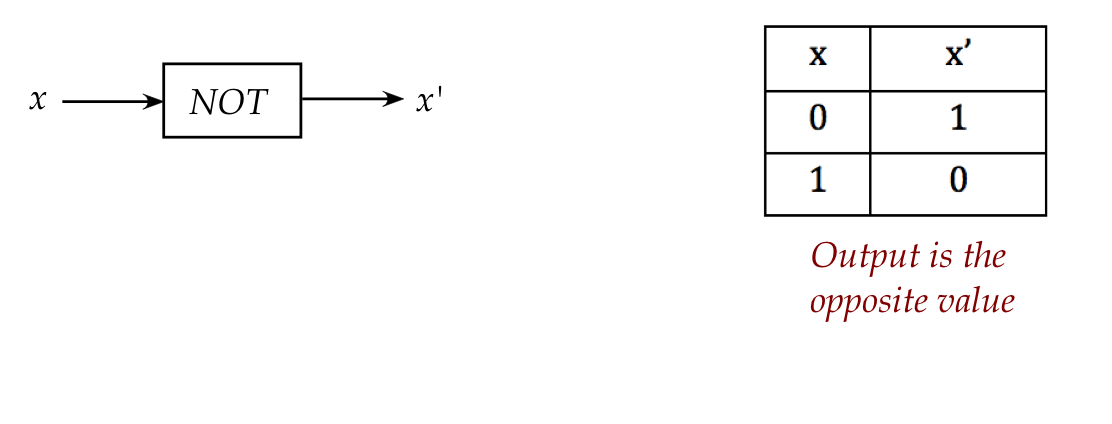
\includegraphics[width=4in]{notes/figs/n10/04classical-not.png}
        \caption{NOT gate}
        \label{fig:04classical-not}
    \end{figure}
    
    We write this as
    
    $$
    \operatorname{NOT}(x)=x^{\prime}
    $$
    
    Next, the classical AND gate shown in Figure \ref{fig:05classical-and}.
    
    \begin{figure}
        \centering
        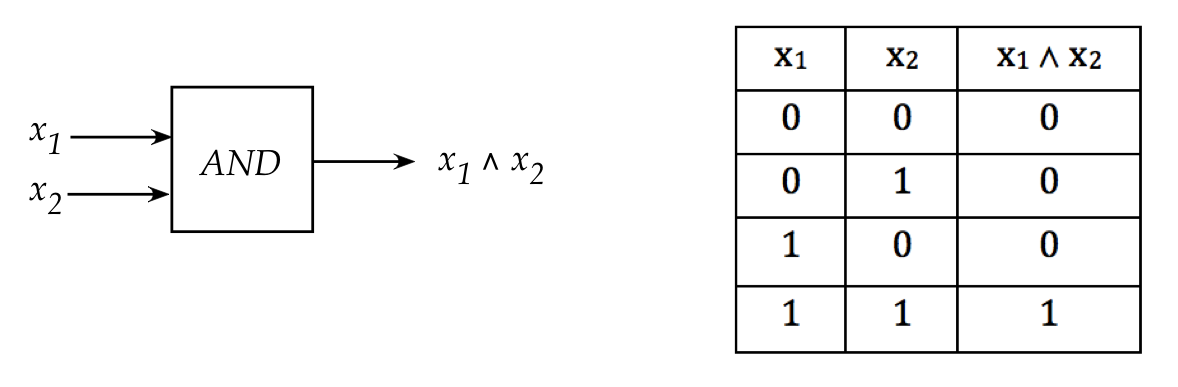
\includegraphics[width=4in]{notes/figs/n10/05classical-and.png}
        \caption{And gate}
        \label{fig:05classical-and}
    \end{figure}
    
    Which we write as any of
    
    $$
    \operatorname{AND}\left(x_{1}, x_{2}\right)=x_{1} \wedge x_{2}=x_{1} x_{2}
    $$
    
    Here, variables like $x_{1}, x_{2}$ are binary variables. Each $x_{i} \in\{0,1\}$. Typically, lower case letters are used. The classical OR gate is shown in Figure \ref{fig:06classical-or}.
    
    \begin{figure}
        \centering
        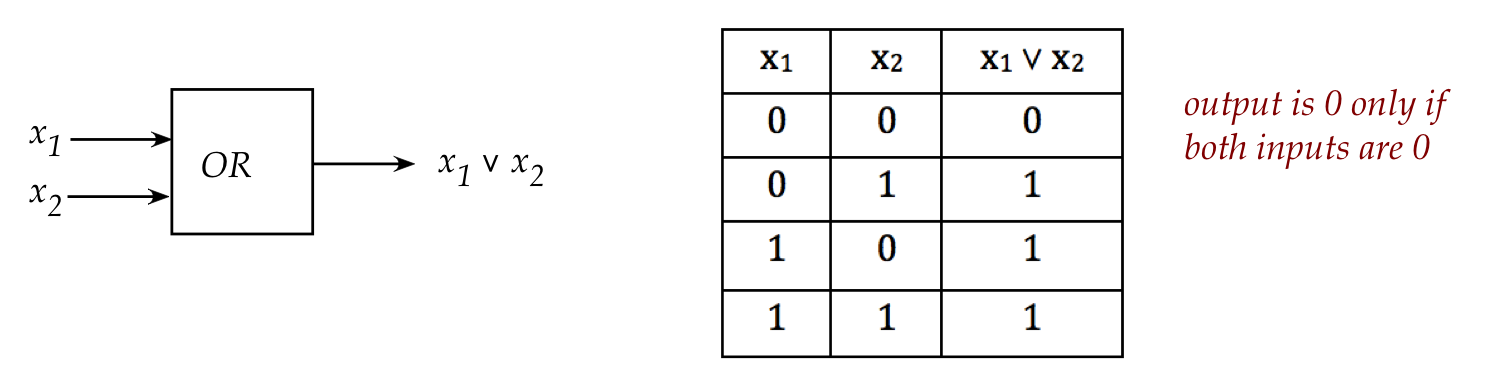
\includegraphics[width=4in]{notes/figs/n10/06classical-or.png}
        \caption{OR gate}
        \label{fig:06classical-or}
    \end{figure}
    
    written symbolically as
    
    $$
    \operatorname{OR}\left(x_{1}, x_{2}\right)=x_{1} \vee x_{2}=x_{1}+x_{2}
    $$
    
    And, an important one for us: the XOR gate shown in Figure \ref{fig:07classical-xor}.
    
    \begin{figure}
        \centering
        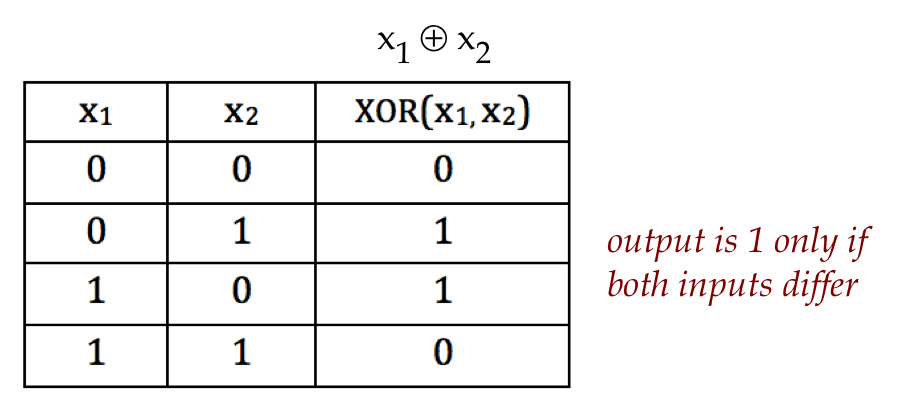
\includegraphics[width=4in]{notes/figs/n10/07classical-xor.png}
        \caption{OR gate}
        \label{fig:07classical-xor}
    \end{figure}
    
    Note the XOR symbol: $x_{1} \oplus x_{2}$. A useful property that XOR shares with AND, OR:
    
    $$
    x_{1} \oplus\left(x_{2} \oplus x_{3}\right)=\left(x_{1} \oplus x_{2}\right) \oplus x_{3}
    $$
    
    So that we can write (unambiguously): $x_{1} \oplus x_{2} \oplus x_{3}$. Also: $x \oplus x=0$. The second use for binary variables is in compactly describing quantum gates: For example, here is a description of the quantum $X$ gate:
    
    $$
    X|a\rangle=\left|a^{\prime}\right\rangle
    $$
    
    Here, $a$ is a binary variable, used only for notational convenience. Thus, when $a=0$
    
    $$
    X|a\rangle=X|0\rangle=\left|0^{\prime}\right\rangle=|1\rangle
    $$
    
    Similarly, when $a=1$
    
    $$
    X|a\rangle=X|1\rangle=\left|1^{\prime}\right\rangle=|0\rangle
    $$
    
    There is no unique way to write such binary-variable descriptions: For example, we could just as easily describe $X$ as:
    
    $$
    X|a\rangle=|1 \oplus a\rangle
    $$
    
    A slightly harder-to-read example:
    
    $$
    H|a\rangle=\frac{1}{\sqrt{2}}\left(|0\rangle+(-1)^{a}|1\rangle\right)
    $$
    
    When $a=0$ :
    
    $$
    H|0\rangle=\frac{1}{\sqrt{2}}\left(|0\rangle+(-1)^{0}|1\rangle\right)=\frac{1}{\sqrt{2}}(|0\rangle+|1\rangle)=|+\rangle
    $$
    
    When $a=1$ :
    
    $$
    H|1\rangle=\frac{1}{\sqrt{2}}\left(|0\rangle+(-1)^{1}|1\rangle\right)=\frac{1}{\sqrt{2}}(|0\rangle-|1\rangle)=|-\rangle
    $$
    
    Note: The notation is used to describe what happens with standard basis vectors: It is these vectors that can be described with binary variables. It may not work with non-binary variables, for example
    
    $$
    X|+\rangle=X \frac{1}{\sqrt{2}}(|0\rangle+|1\rangle)=\frac{1}{\sqrt{2}}(X|0\rangle+X|1\rangle)=|+\rangle
    $$
    
    So, substituting $a=+\operatorname{in} X|a\rangle=\left|a^{\prime}\right\rangle$ does not work. Quantum gates can of course operate on other non-standard-basis inputs. One would need to infer properties for general vectors, such as:
    
    $$
    X(\alpha|0\rangle+\beta|1\rangle)=\beta|0\rangle+\alpha|1\rangle
    $$
    
    The Boolean description is only a notational convenience. It does not mean we are mixing classical and quantum circuits. Let's now describe $C_{N O T}$ (on standard-basis vectors) with this approach:
    
    $$
    C_{N O T}|x, y\rangle=|x, x \oplus y\rangle
    $$
    
    These are the four input cases:
    
    $$
    \begin{array}{|c|c|c|}
    \hline|x\rangle & |y\rangle & |x, x \oplus y\rangle \\
    \hline|0\rangle & |0\rangle & |0,0 \oplus 0\rangle=|00\rangle \\
    |0\rangle & |1\rangle & |0,0 \oplus 1\rangle=|01\rangle \\
    |1\rangle & |0\rangle & |1,1 \oplus 0\rangle=|11\rangle \\
    |1\rangle & |1\rangle & |1,1 \oplus 1\rangle=|10\rangle \\
    \hline
    \end{array}
    $$
    
    Recall the Toffoli $\left(C C_{\text {Nот }}\right)$ gate shown in Figure \ref{fig:08toffoli}.
    
    \begin{figure}
        \centering
        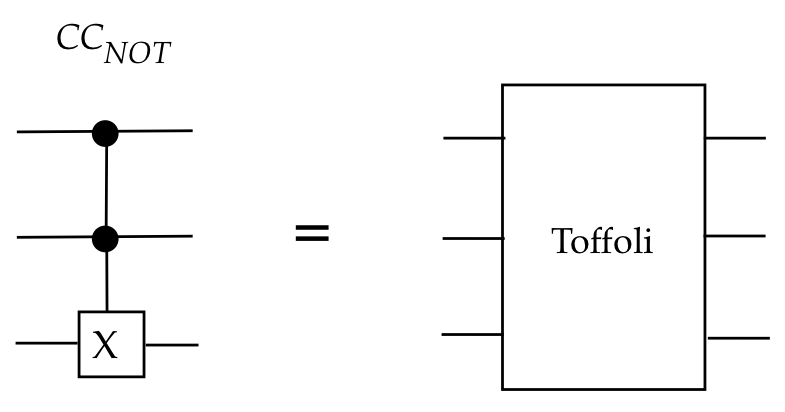
\includegraphics[width=3in]{notes/figs/n10/08toffoli.png}
        \caption{Toffoli}
        \label{fig:08toffoli}
    \end{figure}
    
    The matrix is:
    
    $$
    \left[\begin{array}{llllllll}
    1 & 0 & 0 & 0 & 0 & 0 & 0 & 0 \\
    0 & 1 & 0 & 0 & 0 & 0 & 0 & 0 \\
    0 & 0 & 1 & 0 & 0 & 0 & 0 & 0 \\
    0 & 0 & 0 & 1 & 0 & 0 & 0 & 0 \\
    0 & 0 & 0 & 0 & 1 & 0 & 0 & 0 \\
    0 & 0 & 0 & 0 & 0 & 1 & 0 & 0 \\
    0 & 0 & 0 & 0 & 0 & 0 & 0 & \mathbf{1} \\
    0 & 0 & 0 & 0 & 0 & 0 & \mathbf{1} & 0
    \end{array}\right]
    $$
    
    Algebraically, we describe this as
    
    $$
    \operatorname{TOF}|x, y, z\rangle=|x, y, x y \oplus z\rangle
    $$
    
    Thus, only when $x$ and $y$ are both 1 does $z$ get flipped. Let's use this Boolean-algebraic approach to show that the Toffoli gate is its own inverse:
    
    $$
    \begin{aligned}
    \operatorname{TOF}(\operatorname{TOF}|x, y, z\rangle) &=\operatorname{TOF}(|x, y, x y \oplus z\rangle) \\
    &=|x, y, x y \oplus(x y \oplus z)\rangle \\
    &=|x, y,(x y \oplus x y) \oplus z\rangle \\
    &=|x, y, 0 \oplus z\rangle \\
    &=|x, y, z\rangle
    \end{aligned}
    $$
    
    Similarly, the Fredkin gate can be written as:
    
    $$
    F|x, y, z\rangle=\left|x, x^{\prime} y+x z, x^{\prime} z+x y\right\rangle
    $$
    
    The form is not as simple as the Toffoli gate. The third use of binary variables: naming bits in standard-basis vectors. Consider the 4-qubit vector $|1101\rangle$. We use the notation $\left|b_{3} b_{2} b_{1} b_{0}\right\rangle$ to describe any 4-qubit standard-basis vector. Here, each $b_{i} \in\{0,1\}$ is a binary variable. Thus, with $b_{3}=1, b_{2}=1, b_{1}=0, b_{0}=1$, we get the standard basis vector $|1101\rangle$. In general, an n-qubit standard-basis vector can be written as $\left|b_{n-1} b_{n-2} \ldots b_{1} b_{0}\right\rangle$. Terminology: The leftmost bit is called the most significant bit. And the rightmost, the least significant bit. To see why, consider how the decimal equivalent is built out of the bits:
    
    $$
    k=b_{n-1} 2^{n-1}+b_{n-2} 2^{n-2}+\ldots b_{1} 2^{1}+b_{0} 2^{0}
    $$
    
    For example
    
    $$
    \begin{aligned}
    |1101\rangle &=\left|b_{3} 2^{3}+b_{2} 2^{2}+b_{1} 2^{1}+b_{0} 2^{0}\right\rangle \\
    &=\left|2^{3}+2^{2}+1\right\rangle \\
    &=|13\rangle
    \end{aligned}
    $$
    
    The drawing convention is to place the qubit equivalent to the most significant bit on top shown in Figure \ref{09binary}.
    
    \begin{figure}
        \centering
        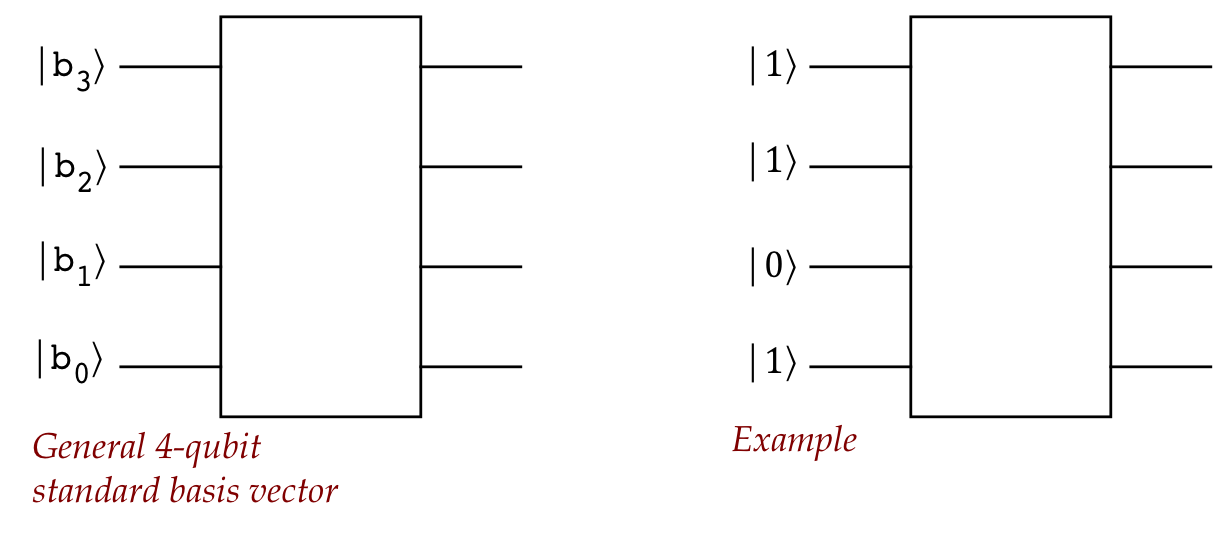
\includegraphics[width=3in]{notes/figs/n10/09binary.png}
        \caption{4-qubit standard basis vector}
        \label{fig:09binary}
    \end{figure}
    
    Bitwise or binary-string operators: It will be useful to extend some operators to binary strings. Let
    
    $$
    \begin{aligned}
    &b=b_{n-1} b_{n-2} \ldots b_{1} b_{0} \\
    &c=c_{n-1} c_{n-2} \ldots c_{1} c_{0}
    \end{aligned}
    $$
    
    represent two binary strings. Then, define:
    
    $$
    \begin{aligned}
    b \wedge c &=b_{n-1} \wedge c_{n-1} \ldots b_{0} \wedge c_{0} \\
    b \oplus c &=b_{n-1} \oplus c_{n-1} \ldots b_{0} \oplus c_{0}
    \end{aligned}
    $$
    
    For example, suppose
    
    $$
    \begin{aligned}
    &b=1011 \\
    &c=1001
    \end{aligned}
    $$
    
    Then
    
    $$
    \begin{aligned}
    &b \wedge c=(1 \wedge 1)(0 \wedge 0)(1 \wedge 0)(1 \wedge 1)=1001 \\
    &b \oplus c=(1 \oplus 1)(0 \oplus 0)(1 \oplus 0)(1 \oplus 1)=0010
    \end{aligned}
    $$
    
    And, it's also convenient to extend the real-vector dot product to binary strings:
    
    $$
    b \cdot c=b_{n-1} c_{n-1}+\ldots+b_{0} c_{0}=\text { Number of common } 1 \text { 's }
    $$
    
    Example:
    
    $$
    1011 \cdot 1001=(1 \cdot 1)+(0 \cdot 0)+(1 \cdot 0)+(1 \cdot 1)=2
    $$
    
    There's a useful variation of the dot product:
    
    $$
    (b \cdot c)_{2}=(b \cdot c) \bmod 2
    $$
    
    Example:
    
    $$
    (1011 \cdot 1001)_{2}=((1 \cdot 1)+(0 \cdot 0)+(1 \cdot 0)+(1 \cdot 1))_{2}=2 \bmod 2=0
    $$
    
    The binary-variable notation enables creating useful algebraic identities, as in this example: Recall how we created the n-qubit all-vector equal superposition from the all-zero input vector:
    
    $$
    (H \otimes H \otimes \ldots \otimes H)|0\rangle|0\rangle \ldots|0\rangle=\frac{1}{\sqrt{N}} \sum_{k=0}^{N-1}|k\rangle
    $$
    
    where $N=2^{n}$ and $k$ is decimal. For example,
    
    $$
    \begin{aligned}
    (H \otimes H)|0\rangle|0\rangle &=\frac{1}{\sqrt{4}} \sum_{k=0}^{3}|k\rangle \\
    &=\frac{1}{\sqrt{4}}(|0\rangle+|1\rangle+|2\rangle+|3\rangle) \\
    &=\frac{1}{2}(|00\rangle+|01\rangle+|10\rangle+|11\rangle)
    \end{aligned}
    $$
    
    Sometimes, this is called the Walsh-Hadamard transform:
    
    $$
    W=H \otimes H \otimes \ldots \otimes H
    $$
    
    and so
    
    $$
    W|00 \ldots 0\rangle=\frac{1}{\sqrt{N}} \sum_{k=0}^{N-1}|k\rangle
    $$
    
    Although $W$ was applied above to $|00 \ldots 0\rangle$ we will want to see what it does to any standard-basis vector. Let $k$ and $m$ be two decimal numbers with binary representation
    
    $$
    \begin{aligned}
    k &=b_{n-1} \ldots b_{0} \triangleq b \\
    m &=c_{n-1} \ldots c_{0} \triangleq c
    \end{aligned}
    $$
    
    where we've defined variables $b, c$ to represent the binary strings $b_{n-1}+\ldots b_{0}$ and $c_{n-1}+\ldots c_{0}$. We'll also use the terms
    
    $$
    \begin{array}{ll}
    k=\operatorname{decimal}(b) & \text { Convert binary string } b \text { to decimal number } k \\
    b=\operatorname{binary}(k) & \text { Binary string } b \text { from decimal number } k
    \end{array}
    $$
    
    Recall that the action of $H$ can be written as
    
    $$
    H|x\rangle=\frac{1}{\sqrt{2}}\left(|0\rangle+(-1)^{x}|1\rangle\right)
    $$
    
    where, on the left, $|x\rangle=|0\rangle$ when $x=0$, and $|x\rangle=|1\rangle$ when $x=1$. Then, noting that the right side basis vectors can be written the same way, with bit strings,
    
    $$
    \begin{aligned}
    H|x\rangle &=\frac{1}{\sqrt{2}}\left((-1)^{0}|0\rangle+(-1)^{x \cdot 1}|1\rangle\right) \\
    &=\frac{1}{\sqrt{2}}\left((-1)^{x \cdot 0}|0\rangle+(-1)^{x \cdot 1}|1\rangle\right) \\
    &=\frac{1}{\sqrt{2}} \sum_{y=0}^{1}(-1)^{x \cdot y}|y\rangle
    \end{aligned}
    $$
    
    Here, we introduced an additional binary variable $y$ for the sum. Then,
    
    $$
    \begin{aligned}
    &W|m\rangle=W\left|c_{n-1}\right\rangle\left|c_{n-2}\right\rangle \ldots\left|c_{1}\right\rangle\left|c_{0}\right\rangle\\
    &=W\left(\left|c_{n-1}\right\rangle \otimes \ldots \otimes\left|c_{0}\right\rangle\right)\\
    &=(H \otimes \ldots \otimes H)\left(\left|c_{n-1}\right\rangle \otimes \ldots \otimes\left|c_{0}\right\rangle\right)\\
    &=H\left|c_{n-1}\right\rangle \otimes \ldots \otimes H\left|c_{0}\right\rangle\\
    &=\frac{1}{\sqrt{2}}\left(|0\rangle+(-1)^{c_{n-1}}|1\rangle\right) \otimes \ldots \otimes \frac{1}{\sqrt{2}}\left(|0\rangle+(-1)^{c_{0}}|1\rangle\right)\\
    &=\frac{1}{\sqrt{2}}\left(\sum_{b_{n-1}=0}^{1}(-1)^{c_{n-1} b_{n-1}}\left|b_{n-1}\right\rangle\right) \otimes \ldots \otimes \frac{1}{\sqrt{2}}\left(\sum_{b_{0}=0}^{1}(-1)^{c_{0} b_{0}}\left|b_{0}\right\rangle\right)\\
    &=\frac{1}{\sqrt{2^{n}}} \sum_{b_{n-1}, \ldots, b_{0}}(-1)^{c_{n-1} \cdot b_{n-1}} \ldots(-1)^{c_{0} \cdot b_{0}}\left(\left|b_{n-1}\right\rangle \otimes \ldots \otimes\left|b_{0}\right\rangle\right)\\
    &=\frac{1}{\sqrt{N}} \sum_{b_{n-1}, \ldots, b_{0}}(-1)^{c \cdot b}\left(\left|b_{n-1} \ldots b_{0}\right\rangle\right)\\
    &=\frac{1}{\sqrt{N}} \sum_{k=0}^{N-1}(-1)^{c \cdot b}|k\rangle
    \end{aligned}
    $$
    
    Note: the $b_{i}$ 's are introduced as binary variables, one for each $i$ and are then "collected" into the binary string $b_{n-1} \ldots b_{0}$, which then got converted to its decimal form $k$. This is useful enough to make a proposition out of it: Proposition 8.1: The action of the Walsh-Hadamard transform on an arbitrary n-qubit basis vector $|m\rangle$ is
   
    $$
    W|m\rangle=\frac{1}{\sqrt{N}} \sum_{k=0}^{N-1}(-1)^{c \cdot b}|k\rangle
    $$
    
    where $c=\operatorname{binary}(m), b=\operatorname{binary}(k)$ and $N=2^{n}$. Application: Many algorithms start with the full-superposition. This result enables their analysis in later stages of an algorithm's circuit.
    

\subsection{Irreversible classical gates and their reversible replacements}

    In this section, we'll focus on classical gates. In places, we'll use the conventions and tools of quantum gates for classical gates (which can, at first, be a little confusing). Let's use the simple XOR gate as an example: Consider this example output in Figure \ref{fig:10xor-gate1}.
    
    \begin{figure}
        \centering
        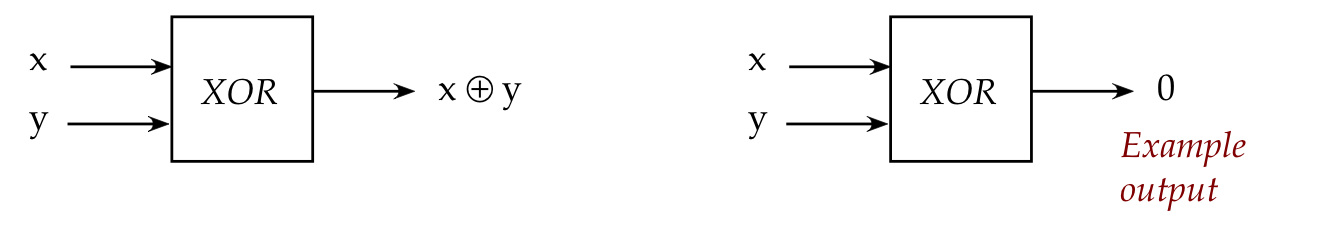
\includegraphics[width=3in]{notes/figs/n10/10xor-gate1.png}
        \caption{XOR Gate}
        \label{fig:10xor-gate1}
    \end{figure}
    
    Looking at the output (0, in this case), one cannot infer the inputs shown in Figure \ref{fig:11xor-gate1b}.
    
    \begin{figure}
        \centering
        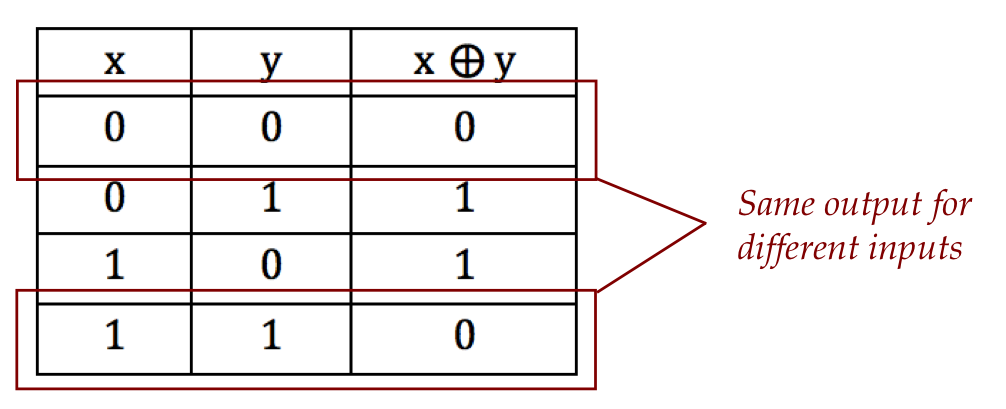
\includegraphics[width=4in]{notes/figs/n10/11xor-gate1b.png}
        \caption{XOR Output}
        \label{fig:11xor-gate1b}
    \end{figure}
    
    Inferring the input is, of course, possible with the NOT gate shown in Figure \ref{fig:12xor-gate2}.
    
    \begin{figure}
        \centering
        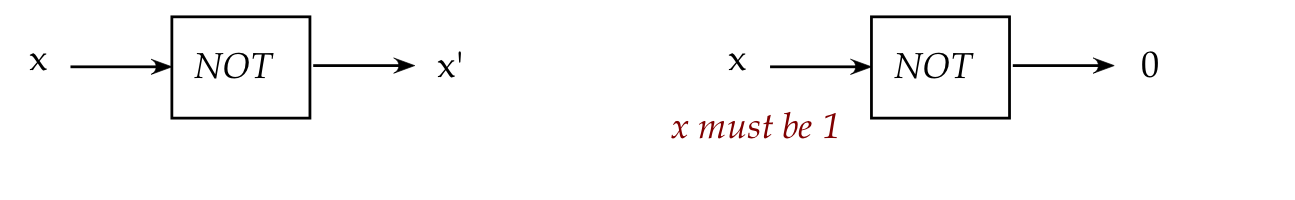
\includegraphics[width=5in]{notes/figs/n10/12xor-gate2.png}
        \caption{NOT Gate}
        \label{fig:12xor-gate2}
    \end{figure}
    
    We say that NOT is reversible while the basic XOR-gate is not reversible. That said, a tiny tweak makes it reversible shown in Figure \ref{fig:13xor-gate3}.
    
    \begin{figure}
        \centering
        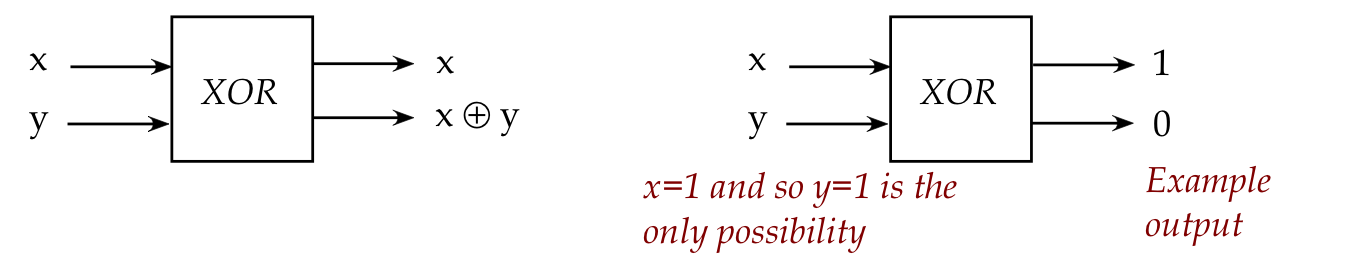
\includegraphics[width=5in]{notes/figs/n10/13xor-gate3.png}
        \caption{XOR reversible}
        \label{fig:13xor-gate3}
    \end{figure}
    
    Here, we have included one of the inputs as an output. Then, knowing the full output (both bits) lets us uniquely infer the inputs. Let's examine the truth-table to clarify shown in Figure \ref{fig:14xor-gate4}.
    
    \begin{figure}
        \centering
        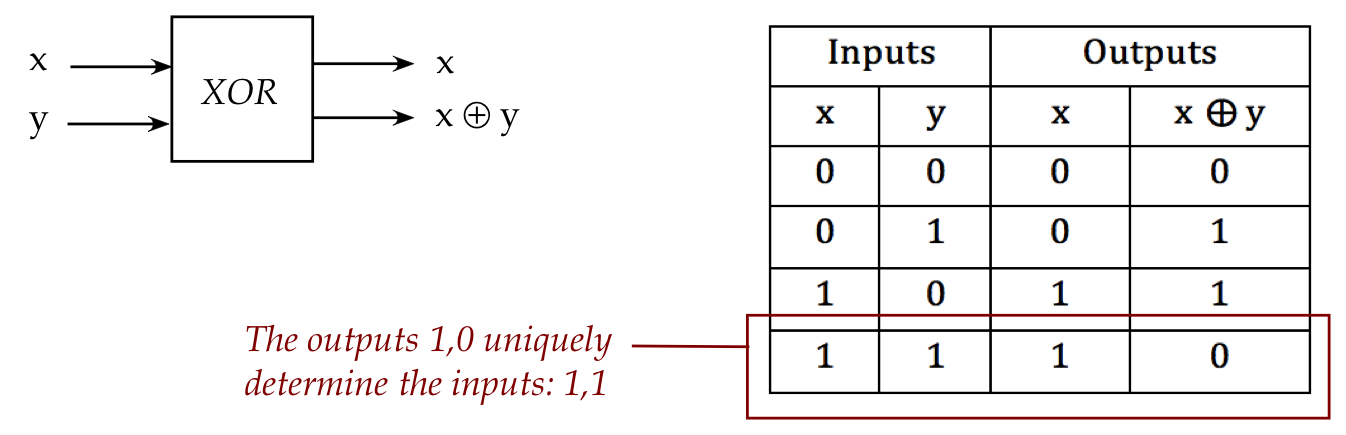
\includegraphics[width=5in]{notes/figs/n10/14xor-gate4.png}
        \caption{XOR reversible truth table}
        \label{fig:14xor-gate4}
    \end{figure}
    
    Each pair of outputs is unique. Thus, the outputs uniquely determine the inputs. We could call this version the XOR-with-x gate. We would find that XOR-with-y is also reversible. We'll now take this idea a step further: We know that all quantum gates are reversible as shown in Figure \ref{fig:15quantum-gate}.
    
    \begin{figure}
        \centering
        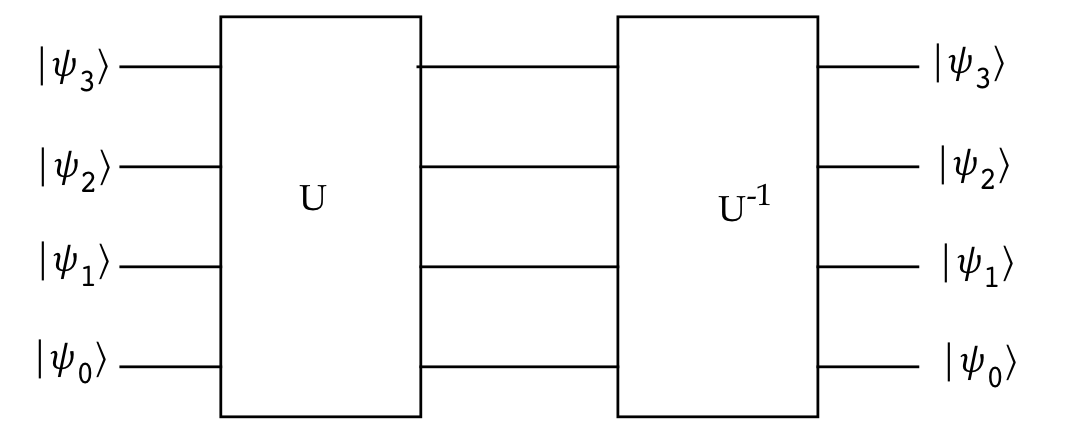
\includegraphics[width=5in]{notes/figs/n10/15quantum-gate.png}
        \caption{reversible quantum gates}
        \label{fig:15quantum-gate}
    \end{figure}
    
    Any quantum gate is a unitary operation $U$. And $U$ has an inverse $U^{-1}=U^{\dagger}$. Thus, applying $U^{\dagger}$ recovers the input. We now ask: can we use the representation (vectors, matrices) for quantum gates for reversible classical gates? Let's try this with the 2-input XOR gate: The four possible inputs are $00,01,10,11$. Suppose we use the same vectors to represent these that we used for $|00\rangle,|01\rangle,|10\rangle,|11\rangle$. That is:
    
    $$
    \text { input } 00=\left[\begin{array}{l}
    1 \\
    0 \\
    0 \\
    0
    \end{array}\right]=|00\rangle \quad \text { input } 01=\left[\begin{array}{l}
    0 \\
    1 \\
    0 \\
    0
    \end{array}\right]=|01\rangle \quad \text { input } 10=\left[\begin{array}{l}
    0 \\
    0 \\
    1 \\
    0
    \end{array}\right]=|10\rangle \quad \text { input } 11=\left[\begin{array}{l}
    0 \\
    0 \\
    0 \\
    1
    \end{array}\right]=|11\rangle
    $$
    
    Note: with classical gates, these are the only inputs and outputs. There are no linear combinations or complex scalars. Next, let's represent the XOR gate by the matrix
    
    $$
    \mathrm{XOR}=\left[\begin{array}{llll}
    1 & 0 & 0 & 0 \\
    0 & 1 & 0 & 0 \\
    0 & 0 & 0 & 1 \\
    0 & 0 & 1 & 0
    \end{array}\right]
    $$
    
    Then
    
    $$
    \begin{array}{lll}
    \text { XOR }|00\rangle=|00\rangle & & \text { Outputs } 0,0 \\
    \text { XOR }|01\rangle=|01\rangle & & \text { Outputs } 0,1 \\
    \text { XOR }|10\rangle=|11\rangle & & \text { Outputs } 1,1 \\
    \text { XOR }|11\rangle=|10\rangle & & \text { Outputs } 1,0
    \end{array}
    $$
    
    $$
    \begin{aligned}
    \text { XOR } &=|00\rangle\langle 00|+| 01\rangle\langle 01|+| 10\rangle\langle 11|+| 11\rangle\langle 10| & \text { Binary } \\
    &=|0\rangle\langle 0|+| 1\rangle\langle 1|+| 2\rangle\langle 3|+| 3\rangle\langle 2| & \text { Decimal }
    \end{aligned}
    $$
    
    How did we derive the matrix? We can examine the input-to-output list above and write out the Dirac form: Alternatively, recall, we can use the sandwich approach and compute each entry $\langle i|X O R| j\rangle$ for $i, j \in\{0,1,2,3\}$ (decimal). A further insight: permutation matrices. A permutation matrix has the property: there is only a single 1 in every row and every column, with all other entries being 0. Such a matrix permutes the elements of a vector, as in
    
    $$
    \left[\begin{array}{llll}
    1 & 0 & 0 & 0 \\
    0 & 0 & 1 & 0 \\
    0 & 1 & 0 & 0 \\
    0 & 0 & 0 & 1
    \end{array}\right]\left[\begin{array}{l}
    a \\
    b \\
    c \\
    d
    \end{array}\right]=\left[\begin{array}{l}
    a \\
    c \\
    b \\
    d
    \end{array}\right]
    $$
    
    Why is this true? Think of the identity matrix has having rows that successively "act" on vector elements: $\triangleright$ Row $k$ of $I$ "picks off" element $v_{k}$ in vector $\mathbf{v}$. A permutation matrix is merely a permutation of the rows of $I$. Thus, if we were to use permutation matrices as classical gates, they would perforce be reversible. For example: we've seen how to do this for XOR. Unfortunately, a 2-input solution does not exist for AND and OR. Using Toffoli as a reversible classical gate: Let's borrow the Toffoli matrix from its quantum equivalent:
    
    $$
    \text { TOF }=\left[\begin{array}{llllllll}
    1 & 0 & 0 & 0 & 0 & 0 & 0 & 0 \\
    0 & 1 & 0 & 0 & 0 & 0 & 0 & 0 \\
    0 & 0 & 1 & 0 & 0 & 0 & 0 & 0 \\
    0 & 0 & 0 & 1 & 0 & 0 & 0 & 0 \\
    0 & 0 & 0 & 0 & 1 & 0 & 0 & 0 \\
    0 & 0 & 0 & 0 & 0 & 0 & 0 & 0 \\
    0 & 0 & 0 & 0 & 0 & 0 & 0 & \mathbf{1} \\
    0 & 0 & 0 & 0 & 0 & 0 & \mathbf{1} & 0
    \end{array}\right]
    $$
    
    We already know that its effect on standard-basis vectors can be described as:
    
    $$
    \operatorname{TOF}|x, y, z\rangle=|x, y, x y \oplus z\rangle
    $$
    
    Now observe that
    
    $$
    \operatorname{TOF}|x, y, 0\rangle=|x, y, x y \oplus 0\rangle=|x, y, x \wedge y\rangle
    $$
    
    Thus, we have a gate that can be used to compute $x \wedge y$ shown in Figure \ref{fig:16toffoli2}.
    
    \begin{figure}
        \centering
        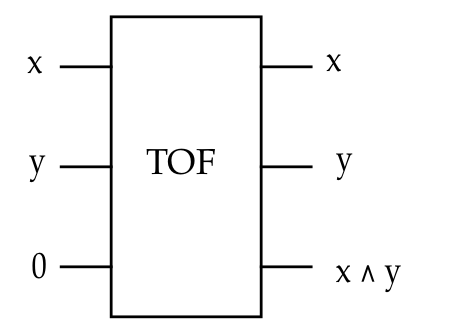
\includegraphics[width=4in]{notes/figs/n10/16toffoli2.png}
        \caption{TOF And}
        \label{fig:16toffoli2}
    \end{figure}
    
    Next, a NOT-gate can be constructed as shown in Figure \ref{fig:17toffoli3}.
    
    \begin{figure}
        \centering
        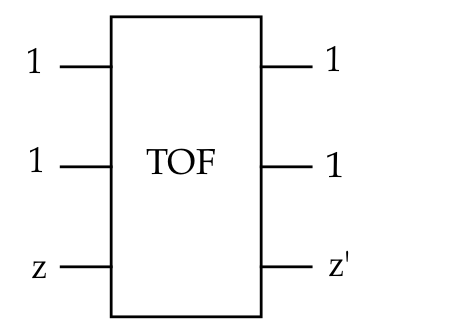
\includegraphics[width=4in]{notes/figs/n10/17toffoli3.png}
        \caption{TOF Not}
        \label{fig:17toffoli3}
    \end{figure}
    
    That is,
    
    $$
    \operatorname{TOF}|1,1, z\rangle=|x=1, y=1,(1 \wedge 1) \oplus z\rangle=\left|1,1, z^{\prime}\right\rangle
    $$
    
    Finally, an OR gate is more complicated: First,
    
    $$
    x \vee y=\left(x^{\prime} \wedge y^{\prime}\right)^{\prime}
    $$
    
    Which we can also write as
    
    $$
    \operatorname{OR}(x, y)=\operatorname{NOT}(\operatorname{AND}(\operatorname{NOT}(x), \operatorname{NOT}(y)))
    $$
    
    Thus, working inwards
    
    $$
    \begin{aligned}
    \operatorname{OR}(x, y) &=\operatorname{TOF}(1,1, \operatorname{AND}(\operatorname{NOT}(x), \operatorname{NOT}(y))) \\
    &=\operatorname{TOF}(1,1, \operatorname{TOF}(\operatorname{NOT}(x), \operatorname{NOT}(y), 0)) \\
    &=\operatorname{TOF}(1,1, \operatorname{TOF}(\operatorname{TOF}(1,1, x), \operatorname{TOF}(1,1, y), 0))
    \end{aligned}
    $$
    
    This is easier to see in a diagram shown in Figure \ref{fig:18toffoli4}.
    
    \begin{figure}
        \centering
        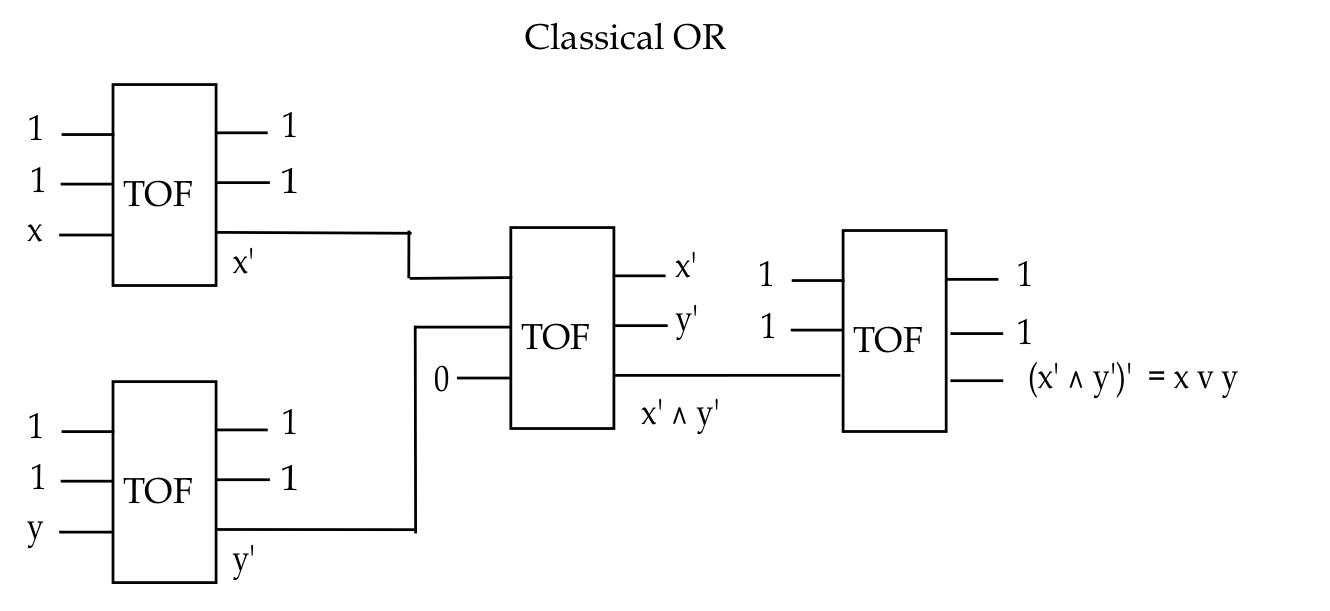
\includegraphics[width=4in]{notes/figs/n10/18toffoli4.png}
        \caption{TOF OR}
        \label{fig:18toffoli4}
    \end{figure}
    
    Thus, the Toffoli gate is universal for classical circuits: Any classical circuit can be built solely out of AND and NOT gates. Each such gate can be replaced by the above Toffoli equivalents, along with extra bits. Note, with NOT gates, one can make the Toffoli-OR circuit a bit more efficient shown in Figure \ref{fig:19toffoli5}.
    
    \begin{figure}
        \centering
        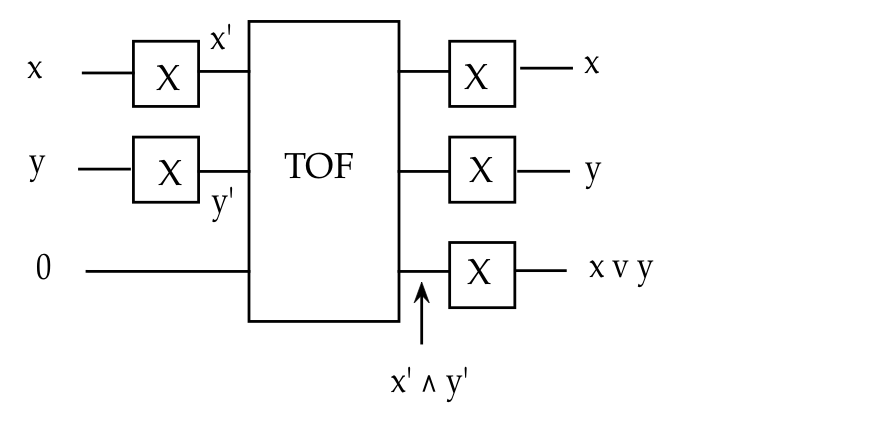
\includegraphics[width=4in]{notes/figs/n10/19toffoli5.png}
        \caption{Efficient Toffoli-OR}
        \label{fig:19toffoli5}
    \end{figure}
    
    What about these extra bits? The spare or extra bits are an additional cost in such an implementation. In a classical circuit, they can just be discarded. However, this discarding cannot easily be done in a quantum circuit because the extra bits may get entangled with the output bits. An alternative: the Fredkin or Controlled-NOT gate shown in Figure \ref{fig:20fredkin}.
    
    \begin{figure}
        \centering
        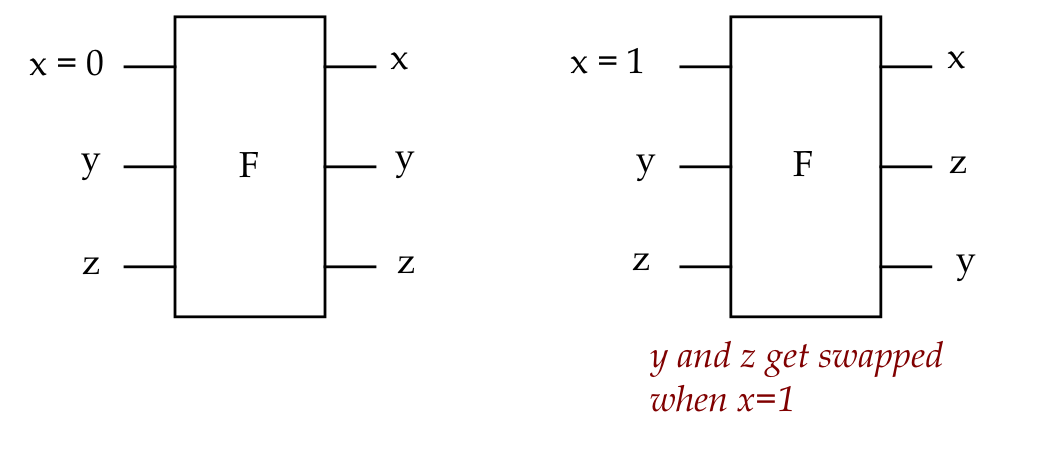
\includegraphics[width=4in]{notes/figs/n10/20fredkin.png}
        \caption{Fredkin}
        \label{fig:20fredkin}
    \end{figure}
    
    We can write the Fredkin algebraically on standard-basis vectors as:
    
    $$
    F|x, y, z\rangle=\left|x, x^{\prime} y+x z, x^{\prime} z+x y\right\rangle
    $$
    
    where $x, y, z$ are all binary variables. Observe that
    
    $$
    F|x, 0,1\rangle=\left|x, x, x^{\prime}\right\rangle
    $$
    
    Thus, the third output can be used as $\operatorname{NOT}(x)$ shown in Figure \ref{fig:21fredkin2}.
    
    \begin{figure}
        \centering
        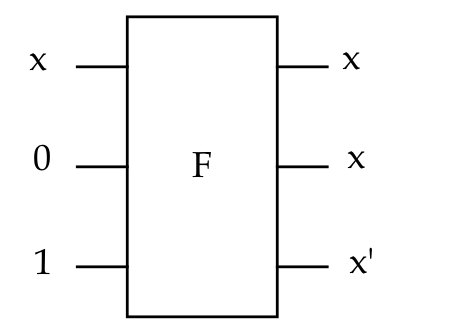
\includegraphics[width=4in]{notes/figs/n10/21fredkin2.png}
        \caption{$\operatorname{NOT}(x)$}
        \label{fig:21fredkin2}
    \end{figure}
    
    The Fredkin gate is also universal: it can implement the NOT, AND, OR classical gates. Recall that the Fredkin is a controlled-SWAP and thus can also be written as:
    
    $$
    F|x, y, z\rangle=\left(I \otimes \operatorname{SWAP}^{x}\right)|x, y, z\rangle=|x\rangle \otimes \operatorname{SWAP}^{x}|y, z\rangle
    $$
    
    where $\operatorname{SWAP}^{0}=I \otimes I$.
    
    The meaning of the classical versions of Toffoli, Fredkin and other such gates: Let's review what we know about qubits and unitary operations: Qubits are hardware devices that can hold a quantum state. A quantum state is represented mathematically by a vector. Qubits are modified by other hardware devices (lasers, magnetic fields, for example). These modifications are mathematically represented by unitary matrices. Now let's review classical circuitry: Bits are stored in flip-flops or 1-bit registers. Each bit is mathematically represented by a binary variable taking a value 0 or 1 . Bits are modified using classical gates like AND, OR, NOT. These are hardware devices that take bits as input and deliver the desired output bits. Classical gates are modeled by Boolean functions. So, what does it mean to represent classical gates with unitary matrices? The idea is to simulate a classical circuit using a quantum circuit. The input to the simulating quantum circuit is a standard-basis vector. Then, if we use the appropriate quantum gates (with Toffoli gates, for example), one can simulate AND and NOT. Then, the output vector can be interpreted as representing a classical-circuit output. Note: the output of the simulating quantum circuit will always be a standard-basis vector because: The input is always a single standard-basis vector. Each unitary is a permutation matrix by design: All the quantum versions of classical gates are permutations. Products and tensors of permutations are permutations. (See section below.) The output is therefore always a standard-basis vector. After designing for standard-basis vectors as input/output, we can of course subject a quantum circuit to superpositions, if that suits our purpose. Cloning with standard basis vectors: While in general cloning is not possible, we can use $C_{NOT}$ gates to clone standard-basis vectors, for example view Figure \ref{fig:22cloning}.
    
    \begin{figure}
        \centering
        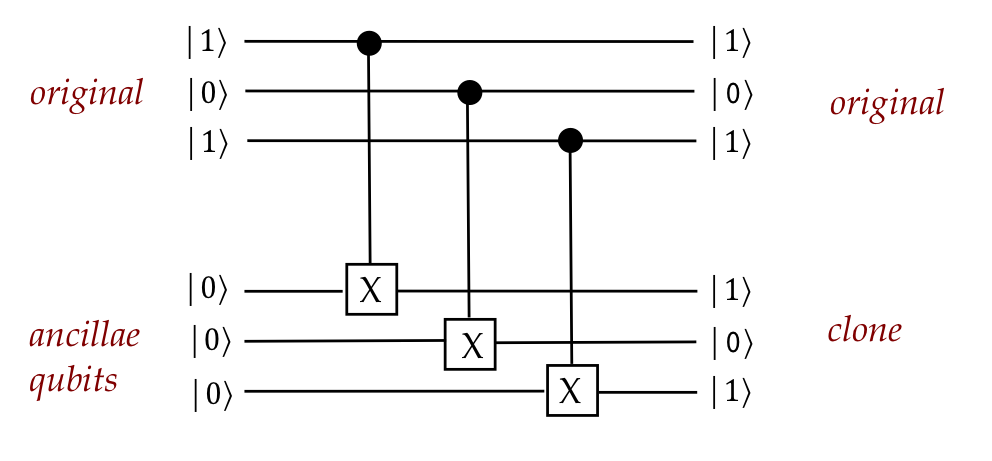
\includegraphics[width=4in]{notes/figs/n10/22cloning.png}
        \caption{$C_{NOT}$ gates to clone standard-basis vectors}
        \label{fig:22cloning}
    \end{figure}

\subsection{An example: half-adder}

    Let's use a simple half-adder to contrast the procedural classical-to-quantum approach with the hand-crafted approach. Let's start with converting classical to quantum: Recall the classical half-adder shown in Figure \ref{fig:23adder1}.
    
    \begin{figure}
        \centering
        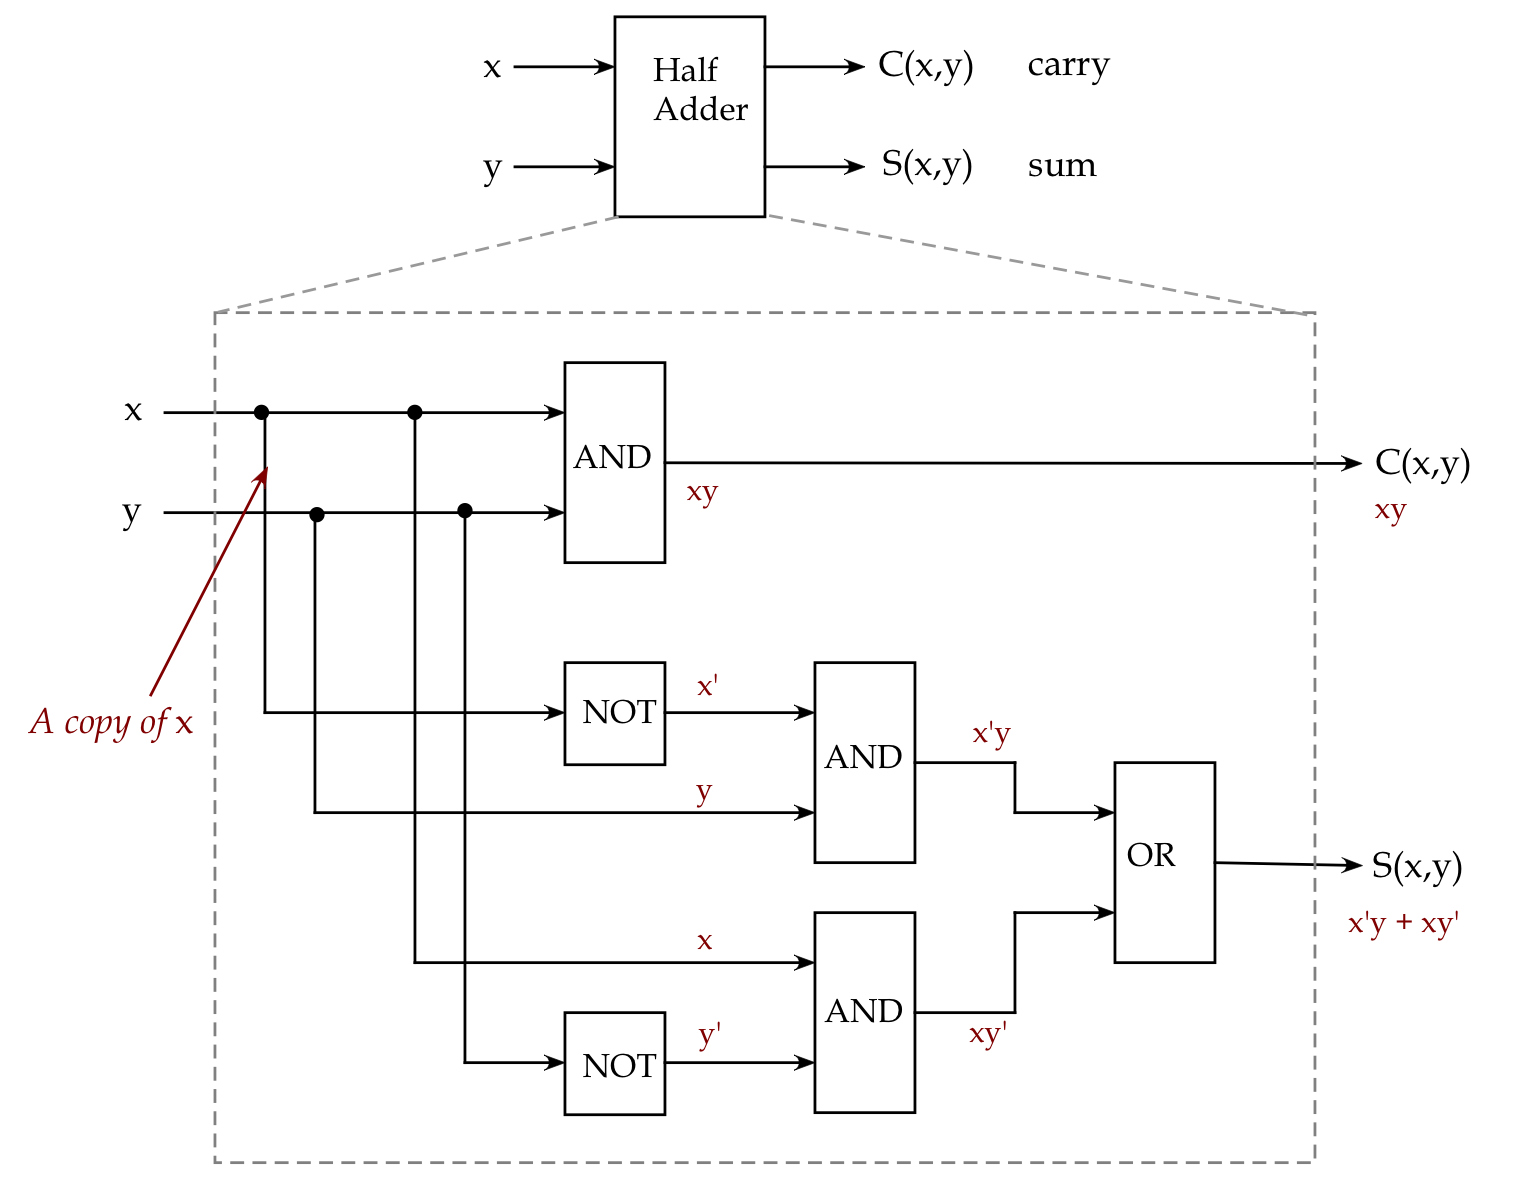
\includegraphics[width=4in]{notes/figs/n10/23adder1.png}
        \caption{Classical Half Adder}
        \label{fig:23adder1}
    \end{figure}
    
    In a purely classical circuit, copying is easy. In a quantum equivalent, we'll need to use $C_{NOT}$ gates. We will build a quantum half-adder using Toffoli, NOT and $C_{NOT}$ gates (for copying). The circuit shown in Figure \ref{fig:24adder2}.
    
    \begin{figure}
        \centering
        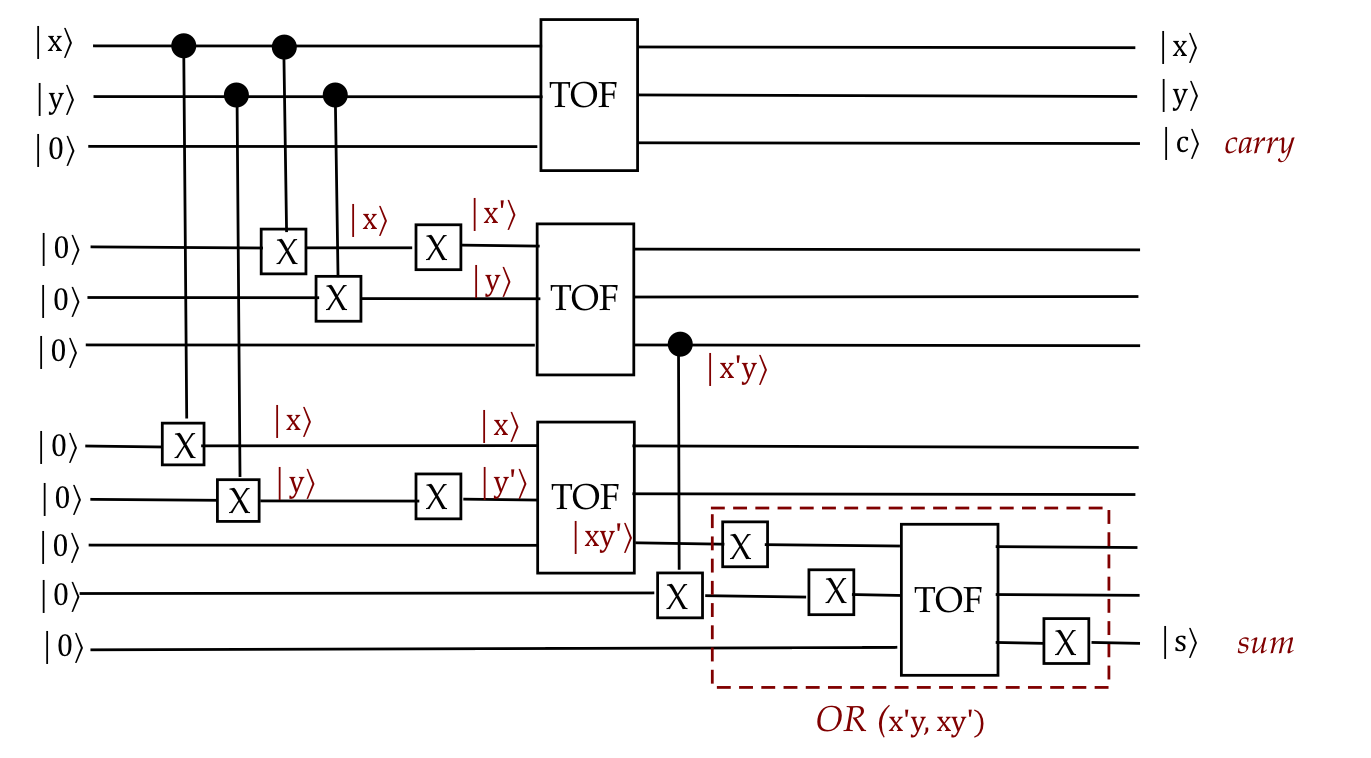
\includegraphics[width=4in]{notes/figs/n10/24adder2.png}
        \caption{quantum half-adder using Toffoli, NOT and $C_{NOT}$ gates}
        \label{fig:24adder2}
    \end{figure}
    
    Let's now contrast this with two clever hand-crafted quantum circuits: Here's a half-adder that's sometimes called the Peres-gate shown in Figure \ref{fig:25adder3}.
    
    \begin{figure}
        \centering
        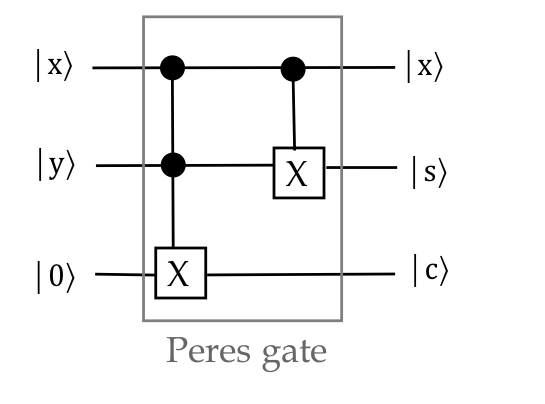
\includegraphics[width=4in]{notes/figs/n10/25adder3.png}
        \caption{Peres-gate}
        \label{fig:25adder3}
    \end{figure}
    
    Algebraically,
    
    $$
    \begin{aligned}
    \left(C_{N O T} \otimes I\right) \mathrm{TOF}|x, y, 0\rangle &=\left(C_{N O T} \otimes I\right)|x, y, x y\rangle \\
    &=C_{N O T}|x, y\rangle \otimes I|x y\rangle \\
    &=|x, x \oplus y\rangle \otimes|x y\rangle \\
    &=|x\rangle|x \oplus y\rangle|x y\rangle
    \end{aligned}
    $$
    
    The sum bit is $|x \oplus y\rangle$. And there's a carry only when $x y=1$. Note: this version overwrites $|y\rangle$. The same idea is easily extended to a full-adder that keeps the input shown in Figure \ref{fig:26adder4}.
    
    \begin{figure}
        \centering
        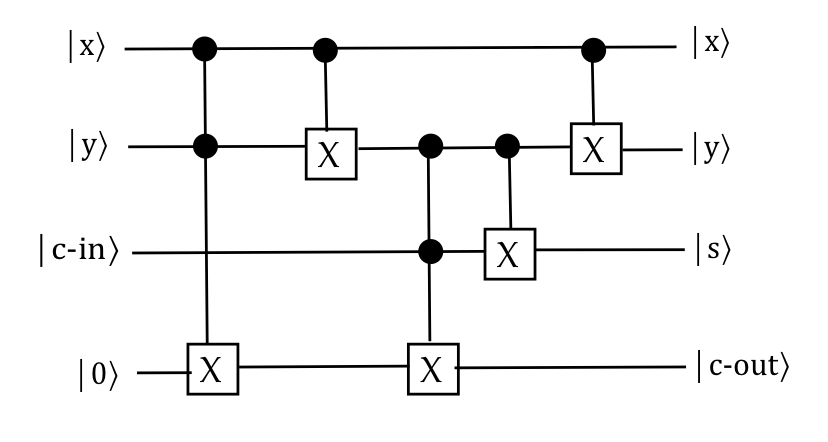
\includegraphics[width=4in]{notes/figs/n10/26adder4.png}
        \caption{full adder}
        \label{fig:26adder4}
    \end{figure}
    
\subsection{Permutations and classical-to-quantum conversion}
    
    Let's examine the connection between reversible classical circuits and permutations. First, let's clarify what mean by a permutation. Let $B_{n}$ be the set of length-n bit strings:
    
    $$
    B_{n}=\left\{x_{n-1} x_{n-2} \ldots x_{1} x_{0}: x_{i} \in\{0,1\}\right\}
    $$
    
    For example:
    
    $$
    B_{3}=\{000,001,010,011,100,101,110,111\}
    $$
    
    Clearly, $\left|B_{n}\right|=2^{n}$. Let $p_{n}$ be a mapping from $B_{n}$ to $B_{n}$ : That is, for any $x \in B_{n}$,
    
    $$
    p_{n}(x) \in B_{n}
    $$
    
    Then $p_{n}$ is a permutation if it is a bijection:
    
    $$
    \forall x \neq x^{\prime}: p_{n}(x) \neq p_{n}\left(x^{\prime}\right)
    $$
    
    That is, for any two inputs, the corresponding outputs are different. One can visualize a permutation as scrambling inputs shown in Figure \ref{fig:27permutation}.
    
    \begin{figure}
        \centering
        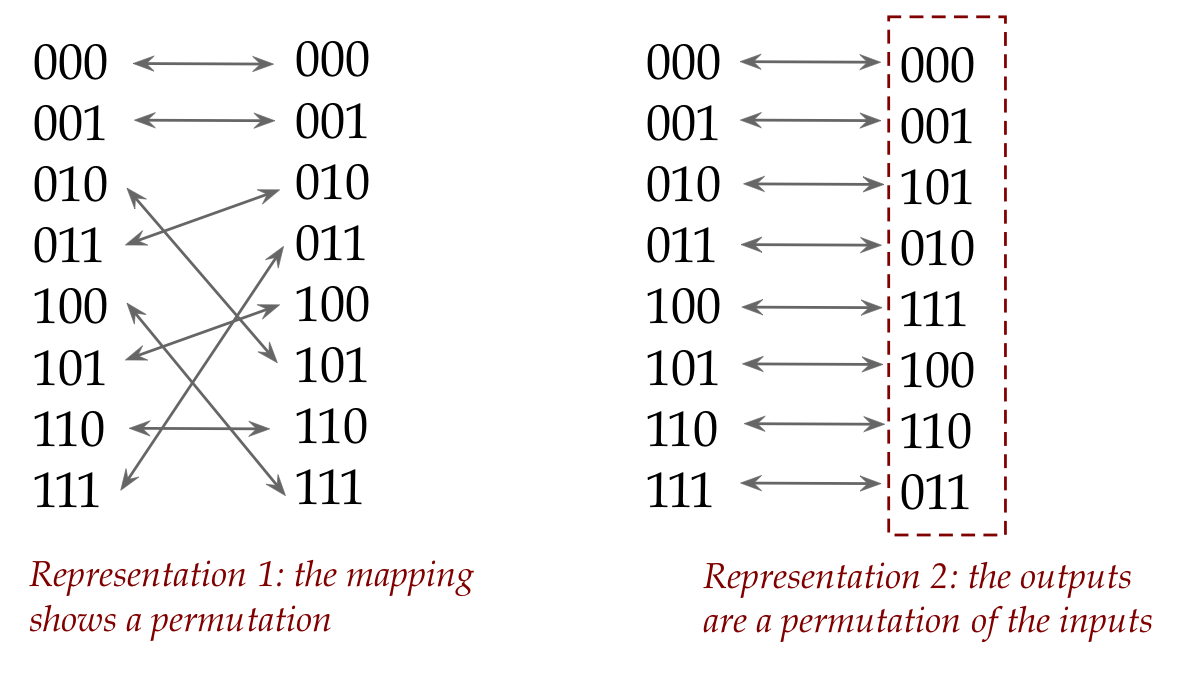
\includegraphics[width=4in]{notes/figs/n10/27permutation.png}
        \caption{permutation}
        \label{fig:27permutation}
    \end{figure}
    
    Note: a permutation is not about permuting the bits in a binary string. Let's vectorize permutations by treating each bit string as representing a standard-basis vector. For example, with $n=2$
    
    $$
    |10\rangle=\left[\begin{array}{l}
    0 \\
    0 \\
    1 \\
    0
    \end{array}\right]
    $$
    
    Then, for every permutation $p_{n}$ there is an equivalent matrix $P_{n}$ such that
    
    $$
    P_{n}|x\rangle=\left|x^{\prime}\right\rangle \quad \text { whenever } p_{n}(x)=x^{\prime}
    $$
    
    We already know how to build such a matrix using outer-products, or the sandwich method. For example, consider the permutation:
    
    $$
    \begin{aligned}
    &|000\rangle \rightarrow|000\rangle \\
    &|001\rangle \rightarrow|001\rangle \\
    &|010\rangle \rightarrow|011\rangle \\
    &|011\rangle \rightarrow|010\rangle \\
    &|100\rangle \rightarrow|101\rangle \\
    &|101\rangle \rightarrow|100\rangle \\
    &|110\rangle \rightarrow|110\rangle \\
    &|111\rangle \rightarrow|111\rangle
    \end{aligned}
    $$
    
    The matrix is formed by the outer-product sum
    
    $$
    \begin{aligned}
    P=&|000\rangle\langle 000|+| 001\rangle\langle 001|+| 010\rangle\langle 011|+| 011\rangle\langle 010|+\\
    &|100\rangle\langle 101|+| 101\rangle\langle 100|+| 110\rangle\langle 110|+| 111\rangle\langle 111|
    \end{aligned}
    $$
    
    Note: we can see the permutation by looking at the right sides of the outer-products: Read the term $|100\rangle\langle 101|$ as "taking 101 to 100 ". because
    
    $$
    |100\rangle\langle 101|| 101\rangle=|100\rangle
    $$
    
    Writing out the matrix results in
    
    $$
    P=\left[\begin{array}{llllllll}
    1 & 0 & 0 & 0 & 0 & 0 & 0 & 0 \\
    0 & 1 & 0 & 0 & 0 & 0 & 0 & 0 \\
    0 & 0 & 0 & 1 & 0 & 0 & 0 & 0 \\
    0 & 0 & 1 & 0 & 0 & 0 & 0 & 0 \\
    0 & 0 & 0 & 0 & 0 & 1 & 0 & 0 \\
    0 & 0 & 0 & 0 & 1 & 0 & 0 & 0 \\
    0 & 0 & 0 & 0 & 0 & 0 & 1 & 0 \\
    0 & 0 & 0 & 0 & 0 & 0 & 0 & 1
    \end{array}\right]
    $$
    
    Clearly, a permutation matrix, by virtue of how we construct it, will result in a matrix where every row and column has only a single $1$. Another way of thinking about a permutation matrix: it's a permutation of the columns (rows) of $I$. We have now equivalenced a reversible classical circuit with a permutation operator. Combining permutation operators: When building larger circuits from smaller ones, we need to know: When two permutations occur in sequence, is the result a permutation?vWhen a permutation is applied to only some qubits, is the result a permutation of the whole? Proposition 8.2: If $P$ and $Q$ are permutation operators, then so is $PQ$. Proof: For two vectors $|x\rangle \neq|y\rangle$, let
    
    $$
    \begin{aligned}
    &\left|x^{\prime}\right\rangle=Q|x\rangle \\
    &\left|y^{\prime}\right\rangle=Q|y\rangle
    \end{aligned}
    $$
    
    We know that $Q|x\rangle \neq Q|y\rangle$ and so $x^{\prime} \neq y^{\prime}$. And because $P$ is a permutation,
    
    $$
    P\left|x^{\prime}\right\rangle \neq P\left|y^{\prime}\right\rangle
    $$
    
    Hence
    
    $$
    P Q|x\rangle \neq P Q|y\rangle
    $$
    
    Proposition 8.3: If $P$ is a permutation operator, then so are $I \otimes P$ and $P \otimes I$.
    Proof: We'll show this for $I \otimes P$. Suppose $I \otimes P$ applies to $n$ qubits. Suppose $I$ applies to the first $k$ qubits, and $P$ apply to the remaining $m$ qubits where $k+m=n$. The key is to observe that any $n$-qubit standard-basis vector $x$ is formed by tensoring lower-size vectors:
    
    $$
    |x\rangle=|v\rangle \otimes|w\rangle
    $$
    
    where $|v\rangle$ is $k$-qubit and $|w\rangle$ is $m$-qubit. Then for any $w \neq w^{\prime}$ we are given that
    
    $$
    P|w\rangle \neq P\left|w^{\prime}\right\rangle
    $$
    
    Thus
    
    $$
    (I \otimes P)|v\rangle \otimes|w\rangle=|v\rangle \otimes P|w\rangle \neq|v\rangle \otimes P\left|w^{\prime}\right\rangle=|v\rangle \otimes\left|w^{\prime}\right\rangle
    $$
    
    Which shows that $I \otimes P$ is a bijection on the standard-basis vectors. What to do if a classical circuit is not a permutation: We already saw an example: AND
    
    $$
    \begin{aligned}
    &|00\rangle \rightarrow |00\rangle \\
    &|01\rangle \rightarrow |00\rangle \\
    &|10\rangle \rightarrow |10\rangle \\
    &|11\rangle \rightarrow |11\rangle
    \end{aligned}
    $$
    
    where the second bit is the binary-AND of the two input bits. Let $|x\rangle$ be an $\mathrm{n}$-qubit vector where $x$ is an $\mathrm{n}$-bit string. Suppose $f(x)$ is a binary-string function where $f(x)$ is an $\mathrm{m}$-bit string. Typically, $m<n$. Often $m=1$ (single bit output). In this case $f(x)$ cannot be a permutation. For example view Figure \ref{fig:28permutation2}.
    
    \begin{figure}
        \centering
        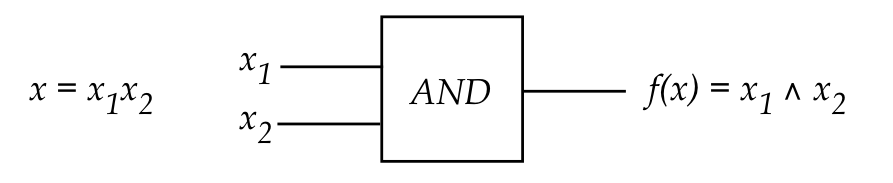
\includegraphics[width=4in]{notes/figs/n10/28permutation2.png}
        \caption{$f(x)$ cannot be a permutation}
        \label{fig:28permutation2}
    \end{figure}
    
    Here, $f(x)=f\left(x_{1}, x_{2}\right)=x_{1} \wedge x_{2}$. This cannot be a permutation. In general, with $m<n$ reference Figure \ref{fig:29permutation3}.
    
    \begin{figure}
        \centering
        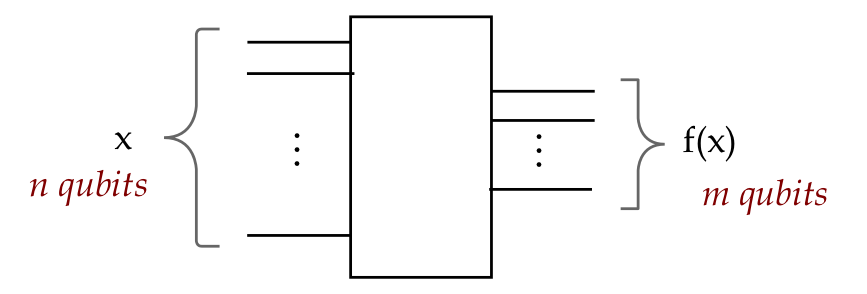
\includegraphics[width=4in]{notes/figs/n10/29permutation3.png}
        \caption{There exist inputs $x$ and $x^{\prime}$ where $f(x)=f\left(x^{\prime}\right)$}
        \label{fig:29permutation3}
    \end{figure}
    
    That is, there exist inputs $x$ and $x^{\prime}$ where $f(x)=f\left(x^{\prime}\right)$. There is a neat trick that equalizes the sizes of inputs/outputs and creates a permutation. First, extend the input into the output shown in Figure \ref{fig:30permutation4}.
    
    \begin{figure}
        \centering
        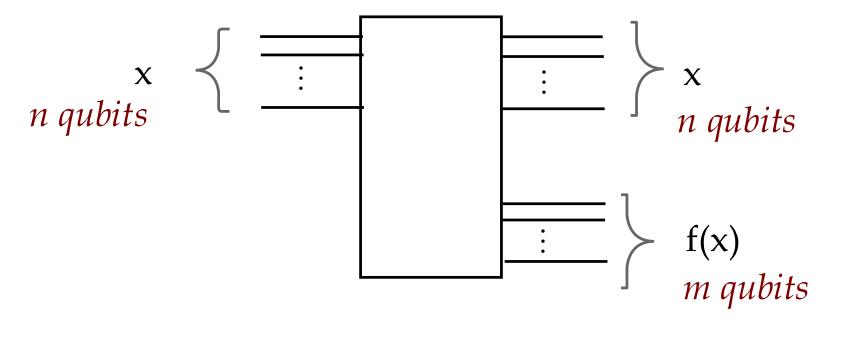
\includegraphics[width=4in]{notes/figs/n10/30permutation4.png}
        \caption{Excess of outputs}
        \label{fig:30permutation4}
    \end{figure}
    
    We now have an excess of outputs. Add additional input lines $y$ to match the $m$ lines for $f(x)$ shown in Figure \ref{fig:31permutation5}.
    
    \begin{figure}
        \centering
        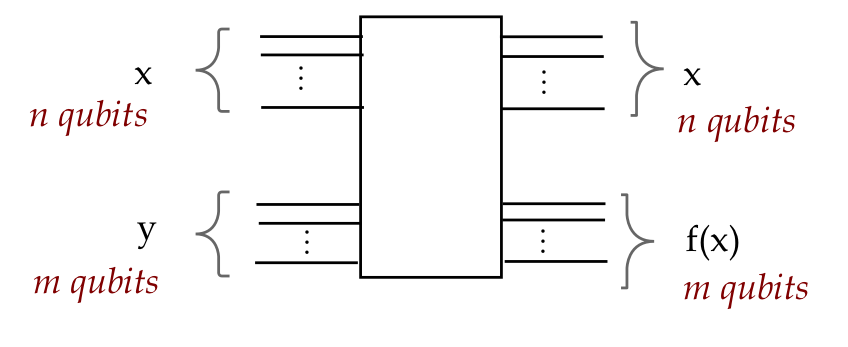
\includegraphics[width=4in]{notes/figs/n10/31permutation5.png}
        \caption{Sizes are matched}
        \label{fig:31permutation5}
    \end{figure}
    
    At this point, the sizes are matched but it's not clear we have a permutation. The next step is to alter the output slightly shown in Figure \ref{fig:32permutation6}.
    
    \begin{figure}
        \centering
        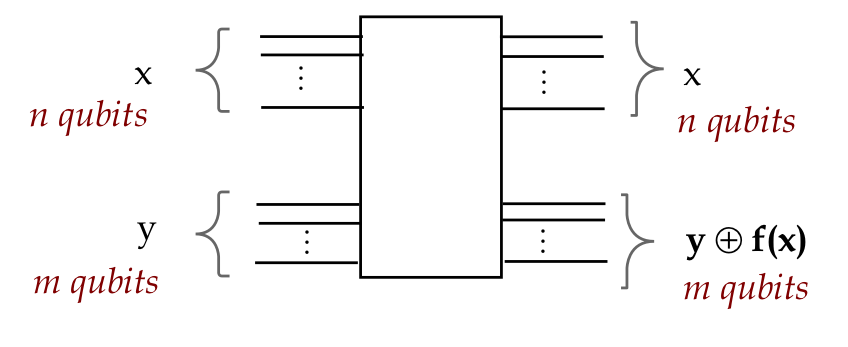
\includegraphics[width=4in]{notes/figs/n10/32permutation6.png}
        \caption{$y \oplus f(x)$}
        \label{fig:32permutation6}
    \end{figure}
    
    Thus the new output is $y \oplus f(x)$. Since this is a classical circuit, we can easily add additional gates to perform the bitwise XOR of $y$ and $f(x)$. To show that this results in a permutation, we'll show that: two different inputs result in two different outputs. Note: The input is the concatenated bit-string $xy$. The output is the concatenated bit-string $x(y \oplus f(x))$. Suppose $x$ and $x^{\prime}$ are different: Then, the inputs $x y$ and $x^{\prime} y$ are different. But so are $x(y \bigoplus f(x))$ and $x^{\prime}\left(y \bigoplus f\left(x^{\prime}\right)\right)$. This is true even if $f(x)=f\left(x^{\prime}\right)$. Suppose $x=x^{\prime}$ and instead $y$ and $y^{\prime}$ are the reason the inputs are different: Then $y$ and $y^{\prime}$ must differ in at least 1 bit. This will result in $y \oplus f(x)$ and $y \oplus f\left(x^{\prime}\right)$ being different on that bit. Thus, the outputs will differ. Let's illustrate the two cases by separating out the part that computes $y \oplus f(x)$ : Case 1: $x \neq x^{\prime}$ shown in Figure \ref{fig:33permutation7}.
    
    \begin{figure}
        \centering
        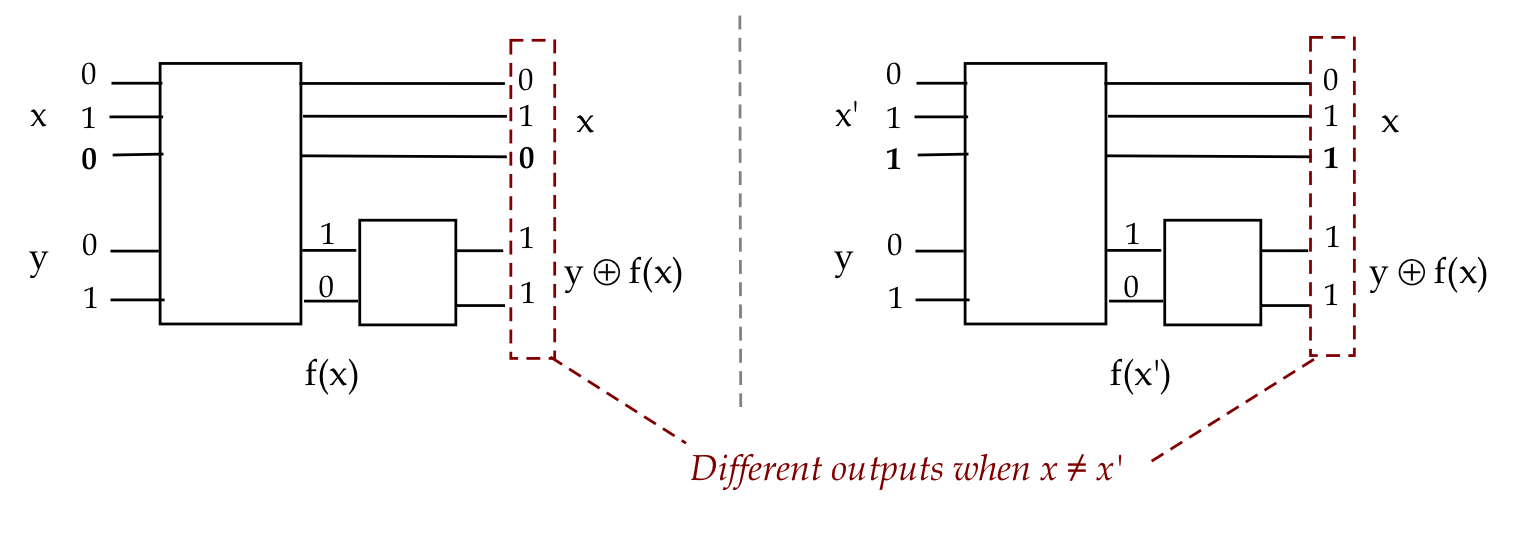
\includegraphics[width=5in]{notes/figs/n10/33permutation7.png}
        \caption{$x \neq x^{\prime}$}
        \label{fig:33permutation7}
    \end{figure}
    
    Case 2: $x=x^{\prime}, y \neq y^{\prime}$ shown in Figure \ref{fig:34permutation8}.
    
    \begin{figure}
        \centering
        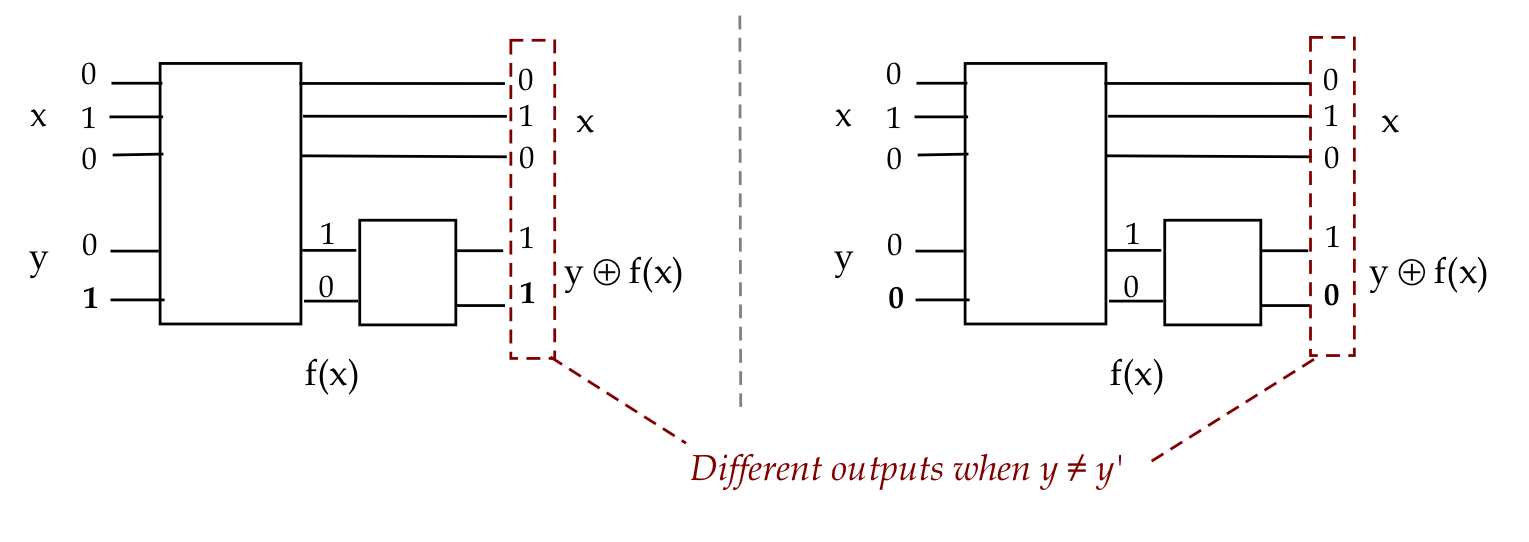
\includegraphics[width=5in]{notes/figs/n10/34permutation8.png}
        \caption{$x=x^{\prime}, y \neq y^{\prime}$}
        \label{fig:34permutation8}
    \end{figure}
    
    This means the entire circuitry can be replaced by a reversible equivalent that performs
    
    $$
    x y \rightarrow x(y \oplus f(x))
    $$
    
    Which we can write vectorially as
    
    $$
    U_{C}|x, y\rangle=|x, y \oplus f(x)\rangle
    $$
    
    where $U_{C}$ is the unitary (reversible) classical permutation operator. However, the original goal of computing $f(x)$ seems thwarted: we are now computing $y \oplus f(x)$. This is easily solved: when we deploying the circuit, we simply feed $y=00 \ldots 0$ (all zeroes), so that
    
    $$
    U|x, 0\rangle=U|x, 0 \oplus f(x)\rangle=|x, f(x)\rangle
    $$
    
    Which is shown in Figure \ref{fig:35permutation9}.
    
    \begin{figure}
        \centering
        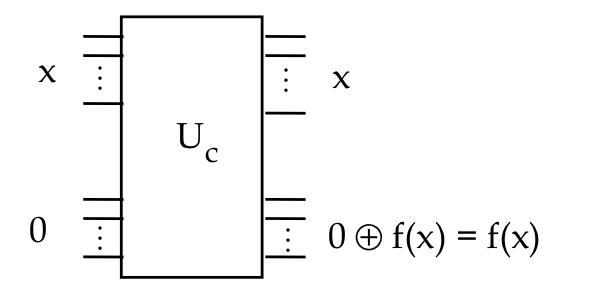
\includegraphics[width=5in]{notes/figs/n10/35permutation9.png}
        \caption{$U|x, 0\rangle=|x, f(x)\rangle$}
        \label{fig:35permutation9}
    \end{figure}
    
    Finally, the quantum equivalent circuit is constructed directly from the unitary matrix shown in Figure \ref{fig:36permutation10}.
    
    \begin{figure}
        \centering
        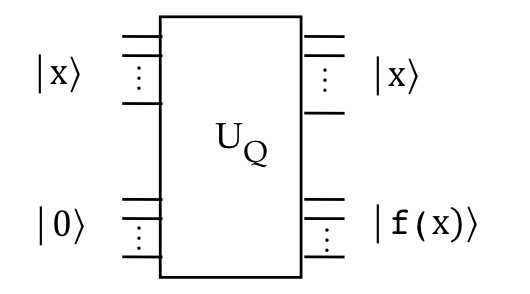
\includegraphics[width=5in]{notes/figs/n10/36permutation10.png}
        \caption{Quantum Equivalent}
        \label{fig:36permutation10}
    \end{figure}
    
    The additional qubits are called ancilla qubits (Plural: ancillae). Let's work through an example with AND: The basic AND gate is not a permutation shown in Figure \ref{fig:37permutation11}.
    
    \begin{figure}
        \centering
        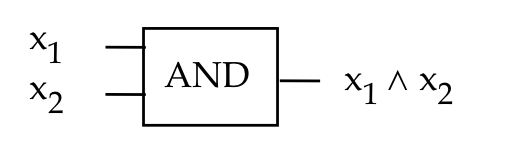
\includegraphics[width=5in]{notes/figs/n10/37permutation11.png}
        \caption{AND Gate}
        \label{fig:37permutation11}
    \end{figure}
    
    We can see this from the truthtable:
    
    \begin{tabular}{|c|c|c|}
    \hline$x_{1}$ & $x_{2}$ & $x_{1} \wedge x_{2}$ \\
    \hline 0 & 0 & 0 \\
    0 & 1 & 0 \\
    1 & 0 & 0 \\
    1 & 1 & 1 \\
    \hline
    \end{tabular}
    
    Now, include $x$ in the output and add $y$ shown in Figure \ref{fig:38permutation12}.
    
    \begin{figure}
        \centering
        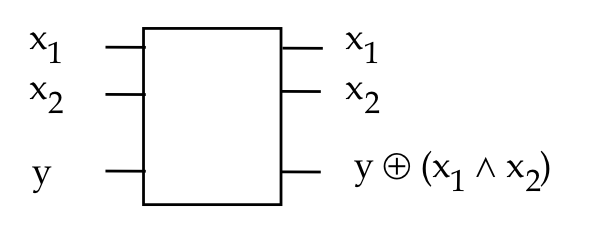
\includegraphics[width=5in]{notes/figs/n10/38permutation12.png}
        \caption{$y \oplus\left(x_{1} \wedge x_{2}\right)$}
        \label{fig:38permutation12}
    \end{figure}
    
    We still haven't figured out the circuit yet. The new truthtable is:
    
    \begin{tabular}{|c|c|c|c|c|c|}
    \hline$x_{1}$ & $x_{2}$ & $y$ & $x_{1}$ & $x_{2}$ & $y \oplus\left(x_{1} \wedge x_{2}\right)$ \\
    \hline 0 & 0 & 0 & 0 & 0 & 0 \\
    0 & 0 & 1 & 0 & 0 & 1 \\
    0 & 1 & 0 & 0 & 1 & 0 \\
    0 & 1 & 1 & 0 & 1 & 1 \\
    1 & 0 & 0 & 1 & 0 & 0 \\
    1 & 0 & 1 & 1 & 0 & 1 \\
    1 & 1 & 0 & 1 & 1 & 1 \\
    1 & 1 & 1 & 1 & 1 & 0 \\
    \hline
    \end{tabular}
    
    The first three columns are the inputs, the second three are outputs. Observe: the last three columns are a permutation (of 3-bit bit strings). We can now write the input-output transformation as:
    
    $$
    \begin{aligned}
    &000 \rightarrow 000 \\
    &001 \rightarrow 001 \\
    &010 \rightarrow 010 \\
    &011 \rightarrow 011 \\
    &100 \rightarrow 100 \\
    &101 \rightarrow 101 \\
    &110 \rightarrow 111 \\
    &111 \rightarrow 110
    \end{aligned}
    $$
    
    When vectorized, this becomes:
    
    $$
    \begin{aligned}
    &|000\rangle \rightarrow|000\rangle \\
    &|001\rangle \rightarrow|001\rangle \\
    &|010\rangle \rightarrow|010\rangle \\
    &|011\rangle \rightarrow|011\rangle \\
    &|100\rangle \rightarrow|100\rangle \\
    &|101\rangle \rightarrow|101\rangle \\
    &|110\rangle \rightarrow|111\rangle \\
    &|111\rangle \rightarrow|110\rangle
    \end{aligned}
    $$
    
    Which means the corresponding operator can be written using a sum of outer-products:
    
    $$
    \begin{aligned}
    P=&|000\rangle\langle 000|+| 001\rangle\langle 001|+| 010\rangle\langle 011|+| 011\rangle\langle 010|+\\
    &|100\rangle\langle 100|+| 101\rangle\langle 101|+| 110\rangle\langle 111|+| 111\rangle\langle 110|
    \end{aligned}
    $$
    
    which in matrix form is:
    
    $$
    \left[\begin{array}{llllllll}
    1 & 0 & 0 & 0 & 0 & 0 & 0 & 0 \\
    0 & 1 & 0 & 0 & 0 & 0 & 0 & 0 \\
    0 & 0 & 1 & 0 & 0 & 0 & 0 & 0 \\
    0 & 0 & 0 & 1 & 0 & 0 & 0 & 0 \\
    0 & 0 & 0 & 0 & 1 & 0 & 0 & 0 \\
    0 & 0 & 0 & 0 & 0 & 1 & 0 & 0 \\
    0 & 0 & 0 & 0 & 0 & 0 & 0 & 1 \\
    0 & 0 & 0 & 0 & 0 & 0 & 1 & 0
    \end{array}\right]
    $$
    
    Unsurprisingly, this is the Toffoli gate or $C C_{NOT}$. In this case, the classical and quantum gates are identical. In other cases, we might get a unitary permutation that is realized in a quantum circuit using prior techniques for decomposing a larger unitary into smaller ones.
    

\subsection{Summary of two approaches: classical to quantum}

    The first approach: Steps: 1. Build the classical circuit with ANDs and NOTs. 2. Optimize classical circuit using classical techniques. 3. Replace ANDs and NOTs with Toffoli gates (still classical). 4. Construct the quantum circuit by using quantum Toffoli gates. Advantages: Classical-circuit optimization is well understood, and has many algorithms. Works well if the quantum hardware has an efficient Toffoli gate. The second approach: Steps: 1. Build classical truth-table $f(x)$ where $x$ is any binary string and $f(x)$ is the binary string output. 2. Convert to permutation and derive permutation (unitary) matrix $U_{f}$ such that
    
    $$
    U_{f}|x, y\rangle=|x, y \oplus f(x)\rangle
    $$
    
    3. Directly optimize and construct quantum circuit. Advantages: Direct quantum circuit construction may be able to exploit characteristics of a given quantum hardware. The output $|0 \oplus f(x)\rangle$ is grouped together, making it convenient to measure or feed into other circuits. For the purposes of algorithm description, we'll use the latter approach.

\subsection{Un-computing}

    Consider the additional qubits needed in a series of unitary transformations: For example, consider two unitary operations $U_{1}, U_{2}$ in sequence shown in Figure \ref{fig:39uncompute}.
    
    \begin{figure}
        \centering
        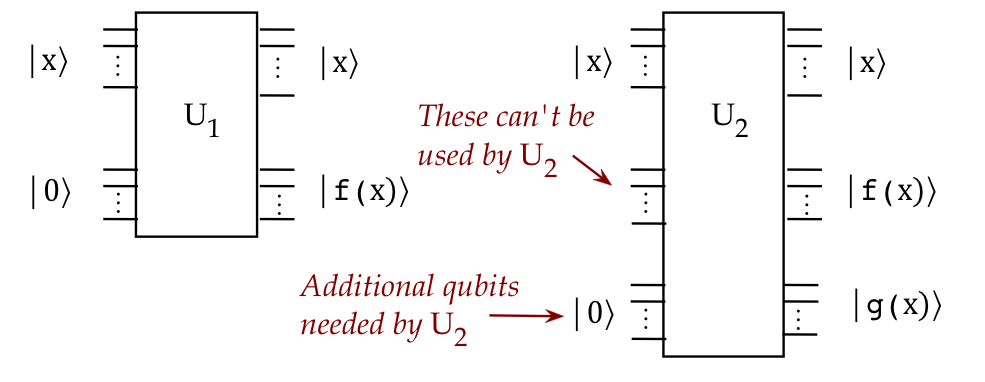
\includegraphics[width=5in]{notes/figs/n10/39uncompute.png}
        \caption{$U_{1}, U_{2}$ in sequence}
        \label{fig:39uncompute}
    \end{figure}
    
    Note: Each of $U_{1}$ and $U_{2}$ need additional qubits for reversible construction. $U_{2}$ applies after $U_{1}$. $U_{2}$ cannot use the same qubits that $U_{1}$ used as ancillae. Couldn't we just "reset" the ancillae qubits? Unfortunately, the output $|f(x)\rangle$ could be entangled with the input $|x\rangle$ that is needed for $U_{2}$. Let's tease this issue out by considering three cases. Consider applying $U$ to a 1-qubit input $|x\rangle$, and 1-qubit output $|f(x)\rangle$. Case 1: the only input is a standard basis vector like $|0\rangle$ or $|1\rangle$ : Then, for example,
    
    $$
    \begin{aligned}
    U|x\rangle|0\rangle &=U|0\rangle|0\rangle & & \text { Example with input }|x\rangle=|0\rangle \\
    &=|0, f(0)\rangle & & \text { Apply } U \text { to produce }|f(x)\rangle \text { in the output } \\
    &=|0\rangle \otimes|f(0)\rangle & & \text { The input is separable }
    \end{aligned}
    $$
    
    Then, measuring $|f(x)\rangle$ or resetting it has no effect on the input, which can be used for further computations. Case 2: A superposition input without entanglement: Let's supply a superposition as the input:
    
    $$
    \begin{aligned}
    U\left(a_{0}|0\rangle+a_{1}|1\rangle\right)|0\rangle &=U\left(a_{0}|0\rangle|0\rangle+a_{1}|1\rangle|0\rangle\right) & & \text { Distribution of tensor over addition } \\
    &=a_{0} U|0\rangle|0\rangle+a_{1} U|1\rangle|0\rangle & & \text { Linearity of } U \\
    &=a_{0}|0, f(0)\rangle+a_{1}|1, f(1)\rangle & & \text { Apply } U \text { to produce }|f(x)\rangle \\
    &=\left(a_{0}|0\rangle+a_{1}|1\rangle\right) \otimes|f(0)\rangle & & \text { Only if } f(0)=f(1)
    \end{aligned}
    $$
    
    Again, in this special instance when $f(0)=f(1)$, the input is separable. Case 3: A superposition that results in entanglement: Suppose $f(0) \neq f(1)$ and that it so happens that $f(0)=0, f(1)=1$. Then,
    
    $$
    \begin{aligned}
    U\left(a_{0}|0\rangle+a_{1}|1\rangle\right)|0\rangle &=a_{0}|0, f(0)\rangle+a_{1}|1, f(1)\rangle & & \text { Apply } U \text { to produce }|f(x)\rangle \\
    &=a_{0}|0,0\rangle+a_{1}|1,1\rangle & & \text { Entangled result }
    \end{aligned}
    $$
    
    In fact, this is a type of Bell vector. Any measurement or resetting of the output will directly affect the input. This, after all, is what the E-91 and teleportation protocols rely on. To get around this problem, the so-called uncompute trick is used: First, recall that standard-basis vectors can in fact be cloned with one $C_{NOT}$ per qubit cloned shown in Figure \ref{fig:40cloning}.
    
    \begin{figure}
        \centering
        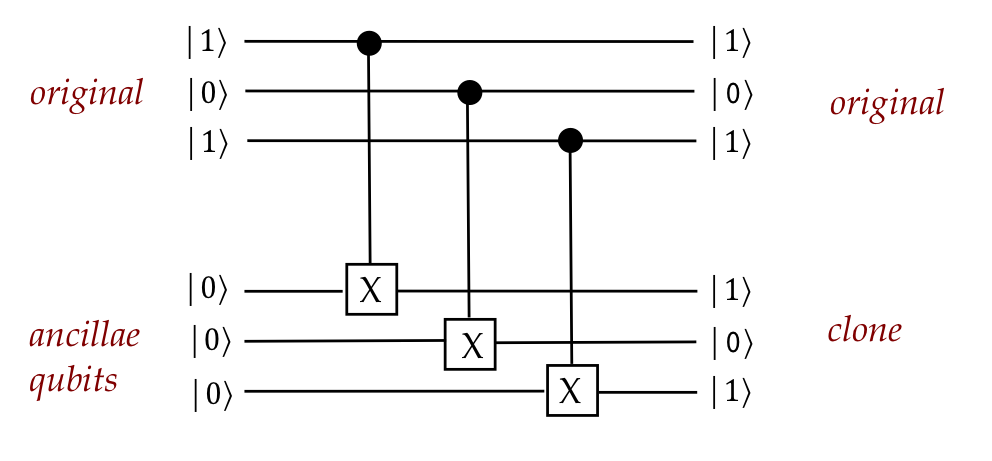
\includegraphics[width=5in]{notes/figs/n10/40cloning.png}
        \caption{standard-basis vectors cloned with one $C_{NOT}$ per qubit cloned}
        \label{fig:40cloning}
    \end{figure}
    
    Next, because any unitary is invertible, we can apply the inverse to restore the original state shown in Figure \ref{fig:41uncompute2}.
    
    \begin{figure}
        \centering
        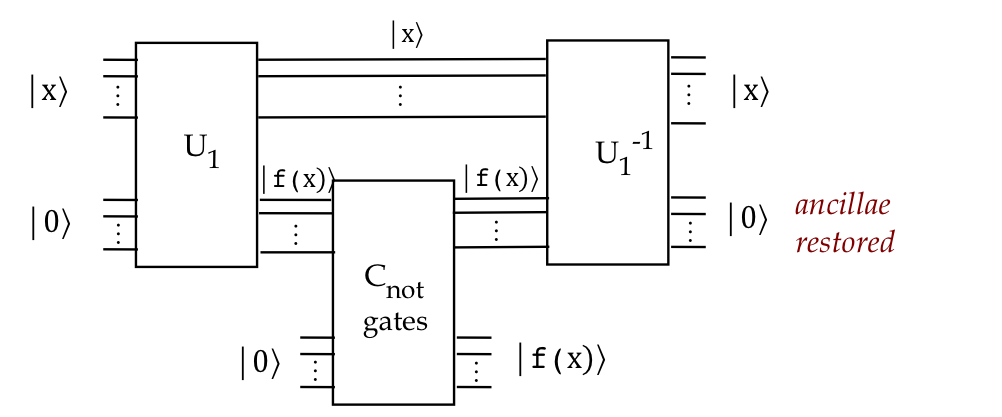
\includegraphics[width=5in]{notes/figs/n10/41uncompute2.png}
        \caption{Apply the inverse}
        \label{fig:41uncompute2}
    \end{figure}
    
    Let's examine this idea algebraically in the multi-qubit case first with a single multi-qubit standard-basis vector $|x\rangle$ as input: Here, $|x\rangle$ and $|f(x)\rangle$ are both multi-qubit. And $|0\rangle$ is short for $|00 \ldots 0\rangle$. We'll use the $C$ to denote the entire $C_{N O T}$-based circuit. Now let's apply all the operators on the full set of qubits:
    
    $$
    \begin{aligned}
    &\left(U_{1}^{-1} \otimes I\right)(I \otimes C)\left(U_{1} \otimes I\right)|x, 0,0\rangle \\
    =&\left(U_{1}^{-1} \otimes I\right)(I \otimes C)|x, f(x), 0\rangle \\
    =&\left(U_{1}^{-1} \otimes I\right)|x, f(x), f(x)\rangle \\
    =&|x, 0, f(x)\rangle \\
    =&|x\rangle|0\rangle|f(x)\rangle
    \end{aligned}
    $$
    
    Next, let's observe that happens when the input is a superposition: In this case we'll want a general input such as
    
    $$\sum_{x} a_{x}|x\rangle$$
    
    where $x$ is a standard-basis bit-string and the $a_{x}$ 's are coefficients.
    
    $$
    \begin{aligned}
    &\left.\left(U_{1}^{-1} \otimes I\right)(I \otimes C)\left(U_{1} \otimes I\right) \mid\left(\sum_{x} a_{x}|x\rangle\right), 0,0\right\rangle \\
    =&\left(U_{1}^{-1} \otimes I\right)(I \otimes C)\left(U_{1} \otimes I\right)\left(\sum_{x} a_{x}|x\rangle \otimes|0\rangle \otimes|0\rangle\right) \\
    =&\left(U_{1}^{-1} \otimes I\right)(I \otimes C)\left(U_{1} \otimes I\right)\left(\sum_{x} a_{x}|x, 0,0\rangle\right) \\
    =&\left(U_{1}^{-1} \otimes I\right)(I \otimes C)\left(\sum_{x} a_{x}\left(U_{1} \otimes I\right)|x, 0,0\rangle\right) \\
    =&\left(U_{1}^{-1} \otimes I\right)(I \otimes C)\left(\sum_{x} a_{x}|x, f(x), 0\rangle\right) \\
    =&\left(U_{1}^{-1} \otimes I\right)\left(\sum_{x} a_{x}(I \otimes C)|x, f(x), 0\rangle\right) \\
    =&\left(U_{1}^{-1} \otimes I\right)\left(\sum_{x} a_{x}|x, f(x), f(x)\rangle\right) \\
    =&\left(\sum_{x} a_{x}\left(U_{1}^{-1} \otimes I\right)|x, f(x), f(x)\rangle\right) \\
    =& \sum_{x} a_{x}|x, 0, f(x)\rangle
    \end{aligned}
    $$
    
    However, because the ancillae are inside the sum, it's not clear that they are disentangled. In fact, they are, although we don't have the algebraic notation to show this. Let's examine the last point more closely with a hypothetical different order, as if we had relabeled the qubits: Consider
    
    $$
    \sum_{x} a_{x}|x, f(x), 0\rangle
    $$
    
    Here, we've merely rearranged the order so that the restored bits are written at the end. Now, we can easily factor out the restored ancillae:
    
    $$
    \sum_{x} a_{x}|x, f(x), 0\rangle=\sum_{x} a_{x}(|x, f(x)\rangle \otimes|0\rangle)=\left(\sum_{x} a_{x}|x, f(x)\rangle\right) \otimes|0\rangle
    $$
    
    Lastly, let's ask why it's important to restore the ancillae: After all, in making a copy of $|f(x)\rangle$, did we not use as many ancillae? The utility arises from performing multiple computations in sequence shown in Figure \ref{fig:42uncompute3}.
    
    \begin{figure}
        \centering
        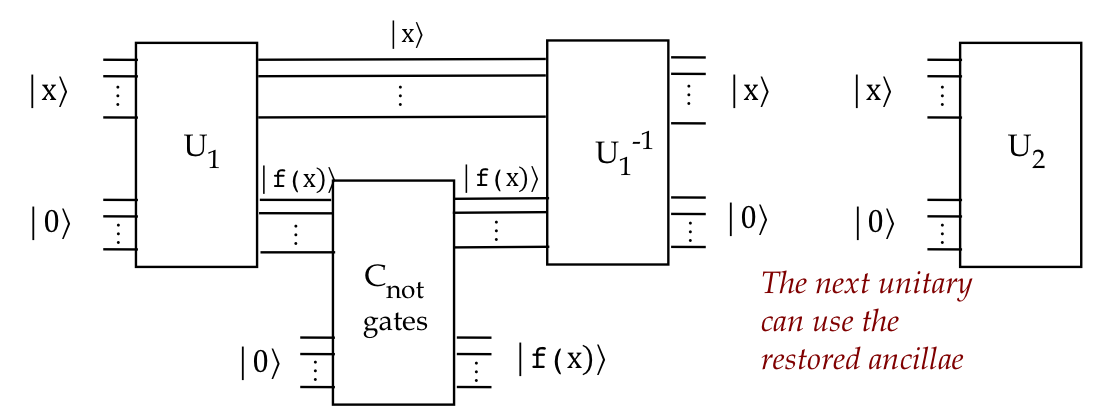
\includegraphics[width=5in]{notes/figs/n10/42uncompute3.png}
        \caption{utility from multiple computations in sequence}
        \label{fig:42uncompute3}
    \end{figure}
    
    Now, later computations can use the restored ancillae. But couldn't $U_{2}$ use the second set of ancillae that fed the $C_{N O T}$ gates? Yes, but presumably $U_{2}$ is some library that's already been optimized with pre-existing assumptions about which ancillae it uses. By having a fixed set of ancillae, sub-units can be optimized accordingly.

\subsection{Efficient reversible classical circuits}

    Quantifiers of efficiency: While the actual time taken on real problems is the ultimate measure, we need some theoretical proxies to analyze algorithms. Two commonly used quantifiers: The total number of qubits, including all ancillae and outputs. The number of small gates. Let's count the added qubits needed when converting a regular classical circuit to a reversible equivalent: After all, this is the key overhead: If the reversible classical one is efficient, so is the quantum equivalent. Let $q=$ the number of classical variables or lines, and $s=$ the number of classical gates. Suppose we assume conversion from a classical non-reversible collection of AND and NOT gates to Toffoli and NOT gates. Replacing each AND with a Toffoli gate needs an additional variable (set to 0 ). In the worst-case, each of the $s$ gates are in their own stage, i.e., $U_{s} U_{s-1} \ldots U_{1}$. In the worst-case, each stage requires as many ancillae as the inputs, or $q$ ancillae. The copying needs an additional $q$ ancillae. Thus, if one did not reuse ancillae, we would need $2 s q$ additional ancillae. However, by carefully reusing ancillae, one can drastically reduce the additional ancillae needed. There is considerable research underway in (classical) design-space algorithms that perform such optimizations.

\end{document}